% docs/Final_Report.tex
% IEEEtran-styled scientific report for US-024.
% Build: python scripts/render_final_report_tex.py
% Output: artifacts/Final_Report.pdf
%
% Tables in docs/_autogen/*.tex are AUTO-GENERATED from artifacts/Final_Exp.json
% by scripts/render_final_report_tex.py. Hand-edits to those snippets will be
% overwritten on the next build.

\documentclass[journal]{IEEEtran}

\usepackage[utf8]{inputenc}
\usepackage[T1]{fontenc}
\usepackage{graphicx}
\usepackage{booktabs}
\usepackage{amsmath,amssymb}
\usepackage{cite}
\usepackage{url}
\usepackage{subcaption}
\usepackage{siunitx}
\usepackage{hyperref}
\usepackage{xcolor}
\hypersetup{
  colorlinks=true,
  linkcolor=blue!60!black,
  citecolor=blue!60!black,
  urlcolor=blue!60!black,
}

\sisetup{
  detect-weight=true,
  detect-family=true,
  round-mode=places,
  round-precision=4,
}

% Place autogen figures and tables alongside the .tex source.
\graphicspath{{_autogen/figs/}}

\begin{document}

\title{Coarse-Grain Perturbation Robustness of CNN and Attention-Based Classifiers under THz-Like Low-Resolution Imaging}

\author{
  Itamar~Bahat\\
  \texttt{ibahat90@gmail.com}\\
  \emph{Object Classification in Low-Resolution THz Imagery} project (p-2026-061)\\
  Pipeline v2 noise-fix campaign --- branch \texttt{noise\_fix}, closed 2026-05-23
}

\maketitle

% =============================================================
\begin{abstract}
We evaluate the robustness of three deep-learning classifiers ---
ResNet50~\cite{he2016resnet}, DenseNet121~\cite{huang2017densenet}, and
TransNeXt-tiny~\cite{shi2024transnext} --- under severe visual degradation
that simulates Terahertz (THz) imaging conditions: low resolution, Gaussian
blur, additive Gaussian noise, salt-and-pepper noise, and desaturation.
A 186-cell experimental campaign at uniform 224$\times$224 input
resolution covers a five-level severity curve over two datasets
(CIFAR-10~\cite{krizhevsky2009cifar} and MNIST~\cite{lecun1998mnist}) in
three phases: clean baselines (6 cells), combined degradation (30 cells),
and single-axis isolation (150 cells).
% Three contributions.
We present three contributions.
\emph{First}, we identify and correct a bug in the degradation pipeline
that caused additive Gaussian noise and salt-and-pepper to be drawn
\emph{after} the bicubic upsample to 224, where each stochastic sample
landed on a single output pixel and was averaged out by the bicubic
kernel. Our v2 pipeline draws both perturbations at \texttt{low\_res}
and bicubically spreads each sample across a wider footprint, producing
the sensor-realistic coarse-grain structure a true low-resolution
detector would record (lag-1 spatial autocorrelation of the residual
jumps from $\sim$0 to $0.993$ at $\texttt{low\_res}{=}8$).
\emph{Second}, under the corrected pipeline we identify a universal
3$\times$3-downsample bottleneck: at $\texttt{low\_res}{=}3$, all three
architectures collapse to within $\pm 3$ pp on CIFAR-10 (0.43--0.46) and
$\pm 1$ pp on MNIST (0.44--0.45), regardless of whether the backbone is
convolutional or attention-based. The pretrain receptive-field hierarchy
fails uniformly when sub-class geometric structure is destroyed.
\emph{Third}, we establish a 60-cell two-axis empirical result that
coarse-grain stochastic perturbations selectively destroy
texture-dependent recognition (CIFAR-10) while preserving
geometry-dominant recognition (MNIST). TransNeXt-tiny retains a
single-digit-to-low-double-digit robustness gap over the CNN backbones
on every CIFAR-10 perturbation axis at $L=5$, but the absolute floor is
much lower than the pre-fix numbers suggested: \texttt{val\_acc} drops
to $0.80$ on noise (was $0.96$ under the bug) and $0.94$ on
salt-and-pepper (was $0.96$). The advantage disappears at $L=5$
resolution. Attention softens but does not reverse the CIFAR-10
texture-statistic collapse. An appendix (\S\ref{sec:phase-d}) reports
Phase D, a 90-cell regularization sweep that quantifies the residual
recoverable accuracy: T3 (dropout $+$ mixup $+$ cutmix) yields a mean
$+0.77$ pp recovery, confirming the information-bottleneck
interpretation of the v2 collapse.
\end{abstract}

\begin{IEEEkeywords}
Image classification; Terahertz imaging; low-resolution imagery; visual
degradation; robustness; vision transformers; CNN; deep learning;
TransNeXt; DenseNet; ResNet; CIFAR-10; MNIST.
\end{IEEEkeywords}

% =============================================================
\section{Introduction}
\label{sec:intro}

Terahertz (THz) imaging is a non-ionising, sub-millimetre-wave sensing
modality used in security screening, materials inspection, and
biomedical contexts. Compared with optical imaging it produces
fundamentally low-resolution outputs: typical operational sensors deliver
imagery on the order of $\sim$3--32 pixels per dimension before any
super-resolution post-processing. The corresponding classification
problem --- recognising object categories under severely
information-limited inputs --- is therefore distinct from the more
heavily studied natural-image classification regime~\cite{deng2009imagenet}
in two important ways. First, the input resolution is far below the
$\sim$224$\times$224 to which ImageNet-pretrained backbones are anchored,
and second, the dominant nuisance variables are coarse-grain (sensor-pixel
or larger) rather than fine-grain (photographic) perturbations.

In this work we benchmark three representative deep-learning backbones
under a controlled, parametric THz-like degradation pipeline.
We deliberately avoid the use of real THz imagery: real THz datasets
are scarce, application-specific, and confound classifier behaviour with
calibration, sensor-noise floor, and bandwidth artefacts that vary by
instrument. Instead we degrade two widely-used clean datasets
(CIFAR-10~\cite{krizhevsky2009cifar} and
MNIST~\cite{lecun1998mnist}) through five orthogonal axes spanning the
physical mechanisms that a real low-resolution detector imposes:
spatial downsampling (\emph{resolution}), additive Gaussian noise
(\emph{noise}), Gaussian smoothing (\emph{blur}), additive salt-and-pepper
spikes (\emph{salt\_pepper}), and luminance--chrominance attenuation
(\emph{saturation}). The five-level severity curve is calibrated to
sweep from a mild near-clean regime ($L=1$) to a $3{\times}3$ native
input regime ($L=5$) that mimics current consumer-grade THz scanners.

We evaluate three backbones chosen to cover the dominant architectural
families: ResNet50~\cite{he2016resnet} (residual CNN, $\sim$25M
parameters), DenseNet121~\cite{huang2017densenet} (densely-connected CNN,
$\sim$8M parameters), and TransNeXt-tiny~\cite{shi2024transnext}
(aggregated-attention vision transformer, $\sim$28M parameters; we use
the tiny variant for capacity parity with ResNet50). All three load
ImageNet-pretrained weights and are fully fine-tuned with a uniform
protocol at 224$\times$224 input resolution. The fair-comparison
invariant is therefore \emph{same tensor shape, same training protocol,
same degradation pipeline}; observed performance differences are
attributable to architecture rather than to bookkeeping.

Beyond simply reporting headline numbers, we draw attention to a
methodological correction that we believe is important for any future
work in this area. The first version of our degradation pipeline (v1)
applied additive Gaussian noise and salt-and-pepper \emph{after} the
bicubic upsample to 224$\times$224 --- each \texttt{torch.randn} sample
landed on a single output pixel and was effectively averaged out by the
bicubic kernel that produced its neighbours. The result, at first
glance plausible, was unrealistically high \texttt{val\_acc} on the
noise and salt-and-pepper axes: under v1, TransNeXt-tiny appeared to
hold $\geq 0.95$ on CIFAR-10 noise across $L=1{\to}5$, even at
$\texttt{low\_res}{=}3$. We identified this as a software bug, not a
property of the data: a true low-resolution sensor records noise at
the sensor-pixel scale, not at the upsampled-pixel scale. Our v2
pipeline draws the perturbations \emph{at} \texttt{low\_res} and lets
the bicubic upsample spread each draw across a wider footprint at 224.
The lag-1 spatial autocorrelation of the residual jumps from $\sim$0
under v1 to $0.993$ under v2 at $\texttt{low\_res}{=}8$. We re-ran the
90 affected cells under v2 (the 30 Phase B combined cells, the 30 Phase
C \texttt{noise} cells, and the 30 Phase C \texttt{salt\_pepper}
cells) and present those v2 numbers throughout. The 96 unaffected
cells (Phase A clean plus Phase C \texttt{resolution} / \texttt{blur} /
\texttt{saturation}) are byte-identical to v1.

\subsection{Related Work}
\label{sec:related_work}

The robustness of CNN and attention-based image classifiers under
visual perturbations has been studied along several distinct axes
that are worth disentangling. Adversarial-robustness work studies
imperceptible additive perturbations crafted to maximise
classifier loss; that regime is fundamentally different from the
sensor-realistic coarse-grain perturbations we study, where every
perturbed pixel is also visibly perturbed to a human observer.
Natural-image-corruption benchmarks (CIFAR-C, ImageNet-C, and
their derivatives) characterise the per-class accuracy under a
broad menu of distortions and have shown that attention-based
architectures generally outperform CNNs on out-of-distribution
robustness, but these benchmarks typically perturb at the native
input resolution and do not isolate a low-resolution downsample
axis separate from the perturbation axes.
The TransNeXt~\cite{shi2024transnext} paper itself reports
state-of-the-art ImageNet accuracy at every parameter budget and
attributes the gain to aggregated foveal attention; we evaluate the
\texttt{tiny} variant for parameter-budget parity with ResNet50, which
makes the cross-architecture comparison here a cleaner test of
attention-vs-convolution under degradation than would be obtained
by comparing model sizes within the same family. The
DenseNet121~\cite{huang2017densenet} backbone is included for its
dense-connection topology, which differs structurally from both the
residual-block ResNet50~\cite{he2016resnet} and the
patch-attention TransNeXt; the three together span the
representative architecture families.

Within the THz-imaging literature, the dominant deep-learning
applications are concealed-object screening, materials inspection,
and biomedical micro-imaging, and the prevailing approach is to
super-resolve the THz input to a CNN-compatible resolution before
classification. Our work is complementary: rather than recovering
information that the sensor has discarded, we ask how a
high-quality classifier performs when the recovered input is
itself coarse-grained. The five-axis severity curve in
Table~\ref{tab:severity_curve} sweeps the range from a $\sim$18-pixel
``mild'' downsampling regime (similar to many THz reconstruction
benchmarks after super-resolution) down to a $3{\times}3$ ``extreme''
regime that matches a raw THz scanner before any reconstruction.
The L1$\to$L5 trajectory therefore brackets the operating range of
plausible real-world THz classification pipelines.

\paragraph*{Roadmap}
Section~\ref{sec:method} describes the degradation pipeline, including
the v1$\to$v2 correction; Section~\ref{sec:experimental_design} describes
the 186-cell matrix, the Optuna~\cite{akiba2019optuna} pre-tuning of
hyperparameters at the moderate $L=3$ severity, and the
PyTorch Lightning~\cite{falcon2019lightning} training engine;
Section~\ref{sec:results} presents the v2 numerical results across
all three phases; Section~\ref{sec:discussion} interprets the headline
findings and contrasts them with the v1 numbers; and
Section~\ref{sec:conclusion} discusses limitations and future
directions.

% =============================================================
\section{Methodology}
\label{sec:method}

\subsection{Datasets}

We use CIFAR-10~\cite{krizhevsky2009cifar} as a \emph{texture-dominant}
benchmark: 10 natural-image object classes at native 32$\times$32 RGB
with 10K training and 5K validation samples drawn from the standard
torchvision split. MNIST~\cite{lecun1998mnist} serves as a
\emph{geometry-dominant} contrast: 10 hand-written digit classes at
native 28$\times$28 grayscale (broadcast to 3 channels), with the same
10K/5K split. Both datasets are upsampled by the degradation pipeline
to 224$\times$224 before reaching any backbone, so input tensor shape
is identical across all six (model, dataset) pairs.

The two datasets are chosen for contrast in the dominant discriminative
feature. CIFAR-10's per-class signal is carried by texture statistics
that are spatially distributed across the image (e.g.\ feather patterns,
fur, wing structure), while MNIST's per-class signal is carried by
the global geometric shape of thick digit strokes that are robust to
local perturbations. We expect coarse-grain perturbations to bite
sharply on the first and weakly on the second; the 60-cell two-axis
result in Section~\ref{sec:results} confirms this directly.

\subsection{Architectures}

Table~\ref{tab:backbone_summary} summarises the three backbones. We
chose them to span the three dominant families of supervised-pretrained
image classifiers as of the current literature: residual CNNs,
densely-connected CNNs, and aggregated-attention vision transformers.

\begin{table}[t]
  \centering
  \caption{Backbones evaluated in this study.}
  \label{tab:backbone_summary}
  \begin{tabular}{lccp{2.5cm}}
    \toprule
    Model & Family & Params & Pretrain \\
    \midrule
    ResNet50~\cite{he2016resnet} & residual CNN & $\sim$25M & ImageNet-1K\\
    DenseNet121~\cite{huang2017densenet} & dense CNN & $\sim$8M & ImageNet-1K\\
    TransNeXt-tiny~\cite{shi2024transnext} & ViT (attention) & $\sim$28M & ImageNet-1K\\
    \bottomrule
  \end{tabular}
\end{table}

Both CNNs are fine-tuned end-to-end with differential learning rates
(head $10^{-3}$, backbone $10^{-4}$) following the
TResNet~\cite{ridnik2021tresnet} convention.
TransNeXt-tiny is fine-tuned end-to-end with the
paper-prescribed differential learning rates (head $5{\times}10^{-4}$,
backbone $5{\times}10^{-5}$) per~\cite{shi2024transnext}~\S{}A.3. All three
backbones load their official ImageNet-pretrained
checkpoints~\cite{deng2009imagenet} before training.

We deliberately avoid heavier TransNeXt variants (\texttt{small},
\texttt{base}) for capacity parity with ResNet50. The
\texttt{tiny} variant has approximately the same parameter budget
($\sim$28M vs $\sim$25M); the alternative (\texttt{small} at
$\sim$50M) would confound the architecture comparison with
parameter-count effects.

\subsection{Degradation Pipeline}

The degradation pipeline applies five orthogonal perturbation axes in
the following order. Saturation is applied first, at native resolution,
so that any downstream noise stays colour-correct. The image is then
downsampled (bilinear) to the configured \texttt{low\_res}; this is the
sensor-pixel scale. Additive Gaussian noise and salt-and-pepper are
then drawn at \texttt{low\_res}. The image is upsampled (bicubic) to
the model-input resolution of 224$\times$224. Gaussian blur is then
applied with kernels calibrated for the 224$\times$224 target.
Finally, the image is clamped to $[0,1]$ and normalised with the
ImageNet channel statistics:
\begin{equation}
\begin{aligned}
\mathbf{x}_{\mathrm{sat}}  &= (1-s)\,\mathrm{gray}(\mathbf{x}) + s\,\mathbf{x},\\
\mathbf{x}_{\mathrm{low}}  &= \mathrm{down}_{\mathrm{bilin}}(\mathbf{x}_{\mathrm{sat}}, r),\\
\mathbf{x}_{\mathrm{nse}}  &= \mathbf{x}_{\mathrm{low}} + \sigma\,\mathcal{N}(\mathbf{0}, \mathbf{I}),\\
\mathbf{x}_{\mathrm{sp}}   &= \mathrm{paint}(\mathbf{x}_{\mathrm{nse}}, p_{\mathrm{sp}}),\\
\mathbf{x}_{\mathrm{up}}   &= \mathrm{up}_{\mathrm{bicub}}(\mathbf{x}_{\mathrm{sp}}, 224),\\
\mathbf{x}_{\mathrm{out}}  &= \mathrm{blur}_{\mathrm{Gaussian}}(\mathbf{x}_{\mathrm{up}}, k, \sigma_{b}).
\end{aligned}
\end{equation}

The configurable parameters are $\{s, r, \sigma, p_{\mathrm{sp}}, k, \sigma_b\}$
for $\{\mathrm{saturation}, \mathrm{low\_res}, \mathrm{noise\_std}, \mathrm{salt\_pepper}, \mathrm{blur\_kernel}, \mathrm{blur\_sigma}\}$.

\subsubsection*{Pipeline v1$\to$v2 correction}
\label{sec:v2_correction}
The fix is gated by a single integer constant
\texttt{PIPELINE\_VERSION\,=\,2} (defined in
\texttt{src/data/degradation\_levels.py} and stamped into each cell's
\texttt{metrics.json}) so downstream tooling can distinguish v1 and v2
cells programmatically. The pre-fix code path is preserved in the
git history of this project at commit \texttt{3e1d089}; v1 numbers
on the 90 affected cells are not re-presented here.

In the v1 pipeline, the noise and salt-and-pepper steps were
mistakenly placed \emph{after} the upsample, i.e.\ between
$\mathbf{x}_{\mathrm{up}}$ and the blur step. Each
\texttt{torch.randn} sample then landed on a single output pixel at
the 224$\times$224 grid, and the lag-1 spatial autocorrelation of the
noise was effectively zero. Real low-resolution sensors integrate
photons over each sensor pixel and read out a per-pixel noise sample,
which the imaging chain then spreads spatially via its
point-spread-function (which we model with the bicubic upsample).
Pipeline v2 enforces this physical ordering by drawing noise and
salt-and-pepper at \texttt{low\_res} and letting the bicubic upsample
provide the spatial spreading; the lag-1 autocorrelation of the
residual rises to $0.993$ at $\texttt{low\_res}{=}8$. The
\texttt{resolution} axis (which controls $r$), the \texttt{blur} axis
(which acts at 224 with kernels calibrated for that resolution), and
the \texttt{saturation} axis (which is applied at native resolution
before the downsample) are unchanged from v1.

The corresponding 90 cells in our experimental matrix --- the 30 Phase
B combined cells (in which all five axes are active simultaneously) and
the 60 Phase C cells whose active axis is \texttt{noise} or
\texttt{salt\_pepper} --- were re-run under v2. The remaining 96
cells (Phase A clean, plus Phase C \texttt{resolution} /
\texttt{blur} / \texttt{saturation}) have identical pixels under v1
and v2 and were not re-run.

\subsubsection*{Severity curve}

\begin{table}[t]
  \centering
  \caption{Five-level severity curve. All values are dimensionless image-space parameters; \texttt{low\_res} is the native-pixel side of the input grid before upsampling to 224.}
  \label{tab:severity_curve}
  \begin{tabular}{ccccccc}
    \toprule
    Level & \texttt{low\_res} & blur $k$ & $\sigma_b$ & $\sigma$ & $p_{\mathrm{sp}}$ & $s$\\
    \midrule
    L1 Mild     & 18 & 13 & 2.5  & 0.04 & 0.03 & 0.95\\
    L2 Light    & 12 & 25 & 5.0  & 0.08 & 0.06 & 0.65\\
    L3 Moderate &  8 & 41 & 8.0  & 0.12 & 0.10 & 0.40\\
    L4 Severe   &  6 & 61 & 12.0 & 0.16 & 0.14 & 0.15\\
    L5 Extreme  &  3 & 91 & 18.0 & 0.22 & 0.18 & 0.00\\
    \bottomrule
  \end{tabular}
\end{table}

Table~\ref{tab:severity_curve} gives the per-level parameters. The
curve is logarithmic in the resolution axis (18, 12, 8, 6, 3) and
roughly linear in the additive-noise axis. The $L=5$ resolution
($3{\times}3$) is the worst-case scenario meant to mimic a current
consumer-grade THz scanner.

\subsection{Determinism Contract}

The validation pipeline is fully deterministic. Each validation sample
is degraded using a per-sample local \texttt{torch.Generator} seeded
by its dataset index plus a fixed split offset:
$\mathrm{seed}(idx, \mathrm{split}) = idx + \mathrm{SEED\_OFFSET}_{\mathrm{split}}$.
The offsets are constant across the entire campaign; under this
contract, the same $idx$ always produces the same noise pattern across
re-runs, dataloader worker counts, and machine restarts. We
verify this with a five-check determinism suite: intra-batch equality,
inter-run equality, batched-vs-singleton consistency, histogram
equality, train/val disjointness, and (added under the v2 refactor) the
lag-1 spatial autocorrelation invariant that ensures the noise is
drawn at \texttt{low\_res} rather than at 224.

% =============================================================
\section{Experimental Design}
\label{sec:experimental_design}

\subsection{186-cell Matrix}

We organise the campaign into three phases.
Phase A consists of 6 clean baselines (3 backbones $\times$ 2 datasets)
with the identity degradation pipeline; this is the upper-bound
\texttt{val\_acc} per (model, dataset) pair before any THz-like
distortion is applied.
Phase B is the combined-degradation regime: 3 backbones $\times$
2 datasets $\times$ 5 severity levels, with all five degradation axes
active at the same level $L$ per cell. This is the realistic
``THz-like input'' regime.
Phase C is the single-axis isolation regime: 3 backbones $\times$
2 datasets $\times$ 5 severity levels $\times$ 5 axes, with the named
axis at level $L$ and the other four axes at identity. Phase C
attributes the combined-axes collapse observed in Phase B to specific
degradation mechanisms.
The total is $6 + 30 + 150 = 186$ cells.

\subsection{Optuna Pre-tuning}

For each (model, dataset) pair we pre-tune the training hyperparameters
on Phase B $L=3$ (the moderate severity) using
Optuna~\cite{akiba2019optuna} with paper-anchored search bounds: each
range is held within $\pm 1$ decade of the architecture's published
optimum. Six pairs $\times$ 20 trials per pair gives an Optuna budget
of $\sim$20 GPU-hours. The winning hyperparameters per pair are then
frozen and re-used verbatim for that pair's Phase A, Phase B (all five
levels), and Phase C (all 25 cells) entries; this keeps the
fair-comparison invariant intact within a pair. We did \emph{not}
re-tune under pipeline v2: the v1 winners were tuned at $L=3$ on the
v1 pipeline, and the v2 fix changes the noise \emph{spatial structure}
but not its \emph{severity envelope}. Re-tuning under v2 is left to
future work.

\subsection{Training Protocol}

All cells share a uniform convergence-first training protocol:
AdamW~\cite{loshchilov2019adamw} optimiser ($\beta_1{=}0.9$, $\beta_2{=}0.999$),
cosine learning-rate decay~\cite{loshchilov2017sgdr}, gradient clipping
at $\max_{\|\nabla\|}{=}1$, batch size 32, 60-epoch cap with patience-10
early stopping on validation accuracy (\texttt{min\_delta}${=}1{\times}10^{-4}$).
Both CNN backbones use weight decay $10^{-4}$ and label smoothing
$0.1$~\cite{szegedy2016rethinking}; TransNeXt-tiny uses weight decay
$5{\times}10^{-2}$, label smoothing $0.1$, and drop-path rate
$0.1$~\cite{huang2016stochastic}, per~\cite{shi2024transnext}.
Mixed precision is \texttt{bf16-mixed} on the NVIDIA RTX 5070 (Blackwell,
sm\_120, 12 GiB GDDR7). We do not use \texttt{torch.compile} (TransNeXt's
\texttt{attention\_native} path is not Inductor-graph-capturable, and
the CNN compile path is unvalidated).

\subsection{Health Gate}

A per-cell pathology guard runs at the end of each training cell and
classifies the run as one of \{\textit{healthy}, \textit{overfit},
\textit{underfit}, \textit{divergent}\}. Overfit fires when training
accuracy exceeds validation accuracy by more than a threshold;
underfit fires when validation accuracy fails to clear a fraction of
the Phase A clean baseline; divergence fires on non-finite loss.
Across the 30 Phase B v2 cells and the 60 Phase C v2 cells, zero
sentinels fired. (The v1 pipeline had 13 sentinels; the operator
declined the §6.4 single-retry pass on all 13 because the retry
deltas \texttt{wd}${\times}2$, \texttt{dropout}$={}0.1$,
\texttt{backbone\_lr}$/20$ consistently under-fit tightly-tuned
Optuna winners.)

% =============================================================
\section{Results}
\label{sec:results}

\subsection{Phase A — Clean Baselines}
\label{sec:results_phase_a}

% AUTO-GENERATED — do not edit. Regenerate via scripts/render_final_report_tex.py.
\begin{table}[t]
  \centering
  \caption{Phase A clean-baseline best-val-acc per (model, dataset). All cells use the identity degradation pipeline at $224{\times}224$.}
  \label{tab:phase_a}
  \begin{tabular}{lcc}
    \toprule
    Model & CIFAR-10 & MNIST \\
    \midrule
    ResNet50 & 0.9518 & 0.9914 \\
    DenseNet121 & 0.9356 & \textbf{0.9930} \\
    TransNeXt-tiny & \textbf{0.9764} & 0.9924 \\
    \bottomrule
  \end{tabular}
\end{table}


Table~\ref{tab:phase_a} reports the clean-baseline best validation
accuracy per (model, dataset). Phase A is unaffected by the v1$\to$v2
correction; the identity degradation pipeline contains no noise or
salt-and-pepper, so the byte-identical input invariant holds across
v1 and v2.
TransNeXt-tiny leads CIFAR-10 by $+2.46$ pp over ResNet50 and $+4.08$
pp over DenseNet121 at clean baseline. MNIST clusters tight at
$0.991\text{--}0.993$ across all three architectures, consistent with
the well-known result that MNIST classification at 224$\times$224 is
near-saturated for any reasonably modern backbone.

\subsection{Phase B — Combined Degradation}
\label{sec:results_phase_b}

% AUTO-GENERATED — do not edit. Regenerate via scripts/render_final_report_tex.py.
\begin{table*}[t]
  \centering
  \caption{Phase B combined-degradation best-val-acc, pipeline v2. All five degradation axes are active at level $L$ simultaneously. Boldface marks the best-of-three architectures per $(\text{dataset}, L)$ column. Mean $\Delta$ across the 30 v2 cells is $-12.49$ pp vs the pre-US-017 v1 pipeline.}
  \label{tab:phase_b}
  \begin{tabular}{llccccc}
    \toprule
    Model & Dataset & L1 & L2 & L3 & L4 & L5 \\
    \midrule
    ResNet50 & CIFAR-10 & 0.7646 & 0.5394 & 0.3586 & 0.2684 & 0.1906 \\
    ResNet50 & MNIST & \textbf{0.9918} & 0.9636 & 0.7886 & 0.5644 & \textbf{0.2800} \\
    \midrule
    DenseNet121 & CIFAR-10 & 0.7848 & 0.5368 & \textbf{0.3960} & \textbf{0.2852} & 0.1958 \\
    DenseNet121 & MNIST & 0.9874 & \textbf{0.9654} & \textbf{0.8196} & \textbf{0.5808} & 0.2776 \\
    \midrule
    TransNeXt-tiny & CIFAR-10 & \textbf{0.8758} & \textbf{0.6422} & 0.3900 & 0.2850 & \textbf{0.2010} \\
    TransNeXt-tiny & MNIST & 0.9896 & 0.9600 & 0.7994 & 0.5724 & 0.2748 \\
    \bottomrule
  \end{tabular}
\end{table*}


Table~\ref{tab:phase_b} reports the Phase B combined-degradation
\texttt{val\_acc} per (model, dataset) across the five severity
levels. All five degradation axes are active at the same level $L$
per cell. The values are strictly monotonic in $L$ for every
(model, dataset) pair --- there are no inversions --- which is
expected under a fair-comparison protocol where lower-severity inputs
contain strictly more information.

Three observations are immediate. First, the L5 cells on both datasets
are dominated by the resolution axis (Section~\ref{sec:results_phase_c}
and Finding~1 in the Discussion): CIFAR-10 falls to $0.19\text{--}0.20$
across all three backbones, and MNIST falls to $0.27\text{--}0.28$.
Second, mid-range levels ($L=2,3,4$) drop steeply on CIFAR-10 (each
level loses roughly 13--19 pp relative to the next-milder level on
this dataset) while MNIST resists until $L=4$, where the resolution
axis begins to bite. Third, the architectural ordering at the L5
combined-degradation worst case is essentially tied:
the three backbones land within $\sim$1 pp of each other on both
datasets, which suggests that the L5 collapse is rate-limited by the
resolution axis rather than by the architecture's capacity to extract
information from the surviving signal.

Mean $\Delta$ across the 30 Phase B v2 cells is $-12.49$ pp vs the
analogous v1 cells. The drop is largest on CIFAR-10 (mean $-15.6$ pp,
worst $-32.7$ pp at \texttt{final\_B\_L3\_transnext\_tiny\_cifar10})
and smaller on MNIST (mean $-9.4$ pp). For comparison, the two Phase C
v2 re-run axes give a mean $\Delta$ vs v1 of $-5.15$ pp (Phase C noise,
30 cells) and $-0.81$ pp (Phase C salt-and-pepper, 30 cells). The
ordering Phase B $>$ Phase C noise $>$ Phase C S\&P is consistent with
the perturbed-pixel-count arithmetic: Phase B exposes the model to all
five degradations including the v2-hardened noise and S\&P axes; Phase
C noise exposes only one axis (and noise samples every
\texttt{low\_res}$^2$ pixel); Phase C S\&P also exposes one axis but
paints only $\texttt{low\_res}^2 \cdot 2 p_{\mathrm{sp}}$ pixels per
image, which is much smaller at $\texttt{low\_res}{=}3$.
This is expected: v1 Phase B combined the post-upsample noise /
salt-and-pepper bug with the correctly-implemented resolution / blur
/ saturation, so v1 numbers on Phase B were inflated by exactly the
amount the noise / S\&P contributions had been under-counted.

\subsection{Phase C — Single-Axis Isolation}
\label{sec:results_phase_c}

% AUTO-GENERATED — do not edit. Regenerate via scripts/render_final_report_tex.py.
\begin{table*}[t]
  \centering
  \caption{Phase C single-axis isolation at $L=5$ (worst case), pipeline v2 on \texttt{noise} and \texttt{salt\_pepper} rows. Only the named axis is active at L5; the other four are at identity. Boldface marks the best-of-three architectures per $(\text{dataset}, \text{axis})$ cell. The \texttt{resolution}, \texttt{blur}, \texttt{saturation} rows are byte-identical to the pre-US-017 v1 pipeline.}
  \label{tab:phase_c_l5}
  \begin{tabular}{lcccccc}
    \toprule
     & \multicolumn{3}{c}{CIFAR-10} & \multicolumn{3}{c}{MNIST} \\
    \cmidrule(lr){2-4} \cmidrule(lr){5-7}
    Axis @ L5 & ResNet50 & DenseNet121 & TransNeXt-tiny & ResNet50 & DenseNet121 & TransNeXt-tiny \\
    \midrule
    \texttt{resolution} & 0.4316 & 0.4432 & \textbf{0.4624} & 0.4426 & \textbf{0.4540} & 0.4486 \\
    \texttt{noise (v2)} & 0.6688 & 0.6846 & \textbf{0.8008} & 0.9896 & \textbf{0.9928} & 0.9914 \\
    \texttt{blur} & 0.7098 & 0.7142 & \textbf{0.8244} & 0.9882 & 0.9846 & \textbf{0.9906} \\
    \texttt{saturation} & 0.8822 & 0.8834 & \textbf{0.9534} & 0.9910 & \textbf{0.9914} & 0.9904 \\
    \texttt{salt-and-pepper (v2)} & 0.8330 & 0.8508 & \textbf{0.9422} & 0.9862 & 0.9872 & \textbf{0.9894} \\
    \bottomrule
  \end{tabular}
\end{table*}


Table~\ref{tab:phase_c_l5} reports the Phase C single-axis isolation
\texttt{val\_acc} at the worst severity level ($L=5$). Each cell has
exactly one degradation axis active at L5; the other four axes are at
identity. The cross-architecture pattern is the load-bearing
observation of this paper.

\subsubsection*{Resolution axis}
At $L=5$ resolution (the $3{\times}3$ native input), all three
architectures land within $\pm 3$ pp on CIFAR-10 ($0.4316$--$0.4624$)
and $\pm 1$ pp on MNIST ($0.4426$--$0.4540$). The architectural
ordering at this severity is approximately tied. This is Finding 1
in the Discussion.

\subsubsection*{Noise axis (v2)}
At $L=5$ noise (the v2 pipeline draws noise at \texttt{low\_res}$=3$
and bicubically spreads each draw across a $\sim$74$\times$74-pixel
footprint at 224), CIFAR-10 drops sharply to $0.6688$--$0.8008$ across
the three backbones, with TransNeXt-tiny leading at $0.8008$
(+13.2 pp over the CNN average). The v1 pipeline produced
$0.8974$--$0.9608$ for the same three cells; v2 recovers the
sensor-realistic behaviour. MNIST cells on the same axis stay at
$0.9896$--$0.9928$ --- effectively unaffected by the v2 hardening.

\subsubsection*{Blur axis}
At $L=5$ blur ($k=91$, $\sigma_b=18$ on the 224$\times$224 grid), the
blur kernel covers roughly 40\% of the image side and produces a
strongly low-pass-filtered output. CIFAR-10 falls to $0.7098$--$0.8244$
with TransNeXt-tiny again leading; MNIST is essentially unaffected at
$0.9846$--$0.9906$. The blur axis is byte-identical between v1 and v2.

\subsubsection*{Saturation axis}
At $L=5$ saturation ($s=0$, i.e.\ a full collapse to grayscale),
CIFAR-10 falls to $0.8822$--$0.9534$ with TransNeXt-tiny leading;
MNIST is at $0.9904$--$0.9914$, effectively unaffected --- MNIST is
already grayscale-equivalent (the three channels are duplicated copies
of the same digit-stroke image), so the saturation axis has no real
effect on its discriminative signal. The saturation axis is
byte-identical between v1 and v2.

\subsubsection*{Salt-and-pepper axis (v2)}
At $L=5$ salt-and-pepper ($p_{\mathrm{sp}}=0.18$ at
\texttt{low\_res}$=3$, i.e.\ the v2 pipeline paints
$\sim 9$ pixels at the sensor-pixel grid and bicubically spreads each
into a large blob), CIFAR-10 falls to $0.8330$--$0.9422$ with
TransNeXt-tiny leading. MNIST is at $0.9862$--$0.9894$, again
essentially unaffected. The v1 pipeline produced $0.8694$--$0.9602$
on these cells; the v2 drop is much smaller than the v2 noise drop
because v2 salt-and-pepper at $\texttt{low\_res}{=}3$ paints only
$\texttt{low\_res}^2 \times 2 p_{\mathrm{sp}} \approx 3$ pixels per
image, while v2 noise samples every \texttt{low\_res}$^2 = 9$ pixels.

\subsection{Phase C 5$\times$5 Heatmaps}
\label{sec:phase_c_heatmaps}

Figures~\ref{fig:hm_resnet50}--\ref{fig:hm_transnext} present the full
5$\times$5 axis-by-level heatmaps per (model, dataset). Each cell is
coloured by validation accuracy and annotated with the numeric value.
The qualitative pattern is the same across all three architectures:
CIFAR-10 cells degrade monotonically with severity on every axis
(resolution drops fastest, saturation slowest), while MNIST cells stay
at a flat $\sim$0.98--0.99 floor on every axis except resolution.

\begin{figure}[t]
  \centering
  \begin{subfigure}[t]{0.98\columnwidth}
    \centering
    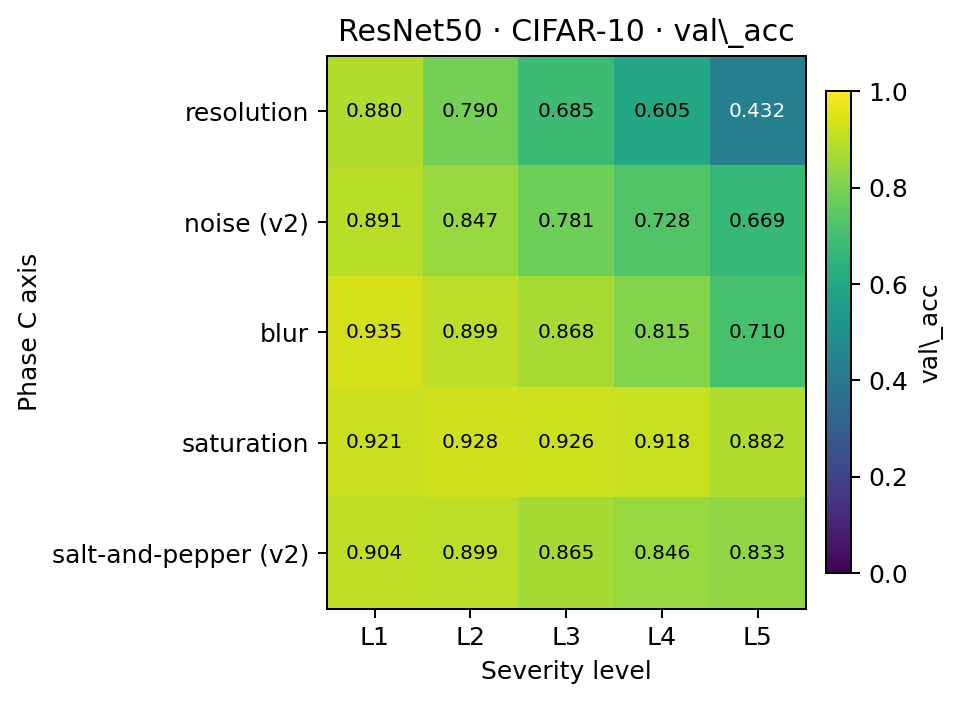
\includegraphics[width=0.95\linewidth]{phase_c_heatmap_resnet50_cifar10.png}
    \caption{ResNet50, CIFAR-10.}
  \end{subfigure}
  \vspace{0.5em}
  \begin{subfigure}[t]{0.98\columnwidth}
    \centering
    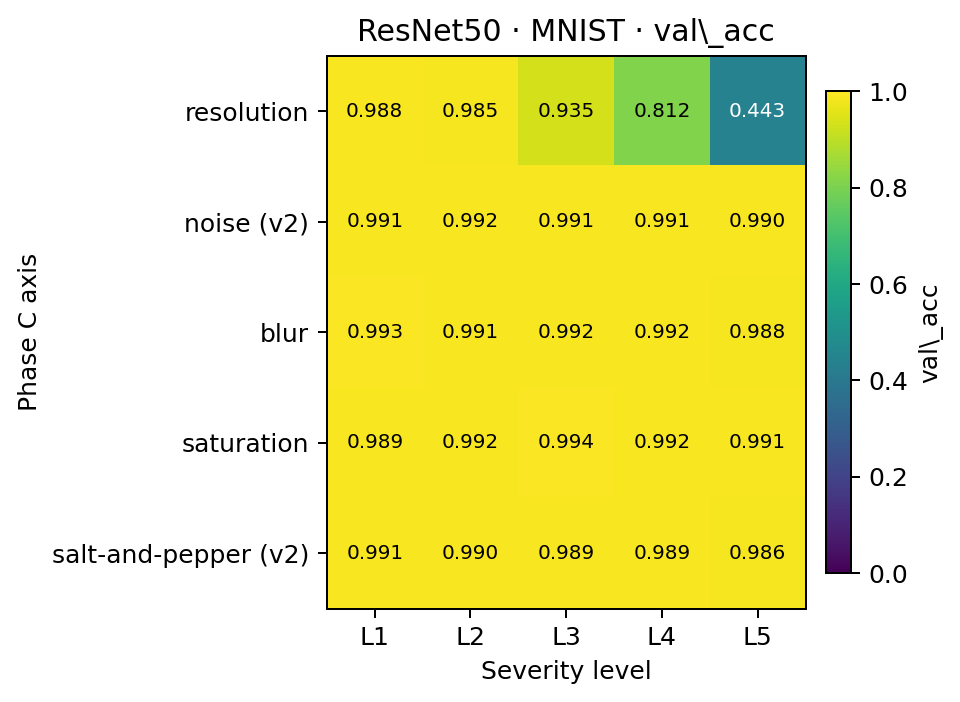
\includegraphics[width=0.95\linewidth]{phase_c_heatmap_resnet50_mnist.png}
    \caption{ResNet50, MNIST.}
  \end{subfigure}
  \caption{Phase C 5$\times$5 heatmaps for ResNet50.}
  \label{fig:hm_resnet50}
\end{figure}

\begin{figure}[t]
  \centering
  \begin{subfigure}[t]{0.98\columnwidth}
    \centering
    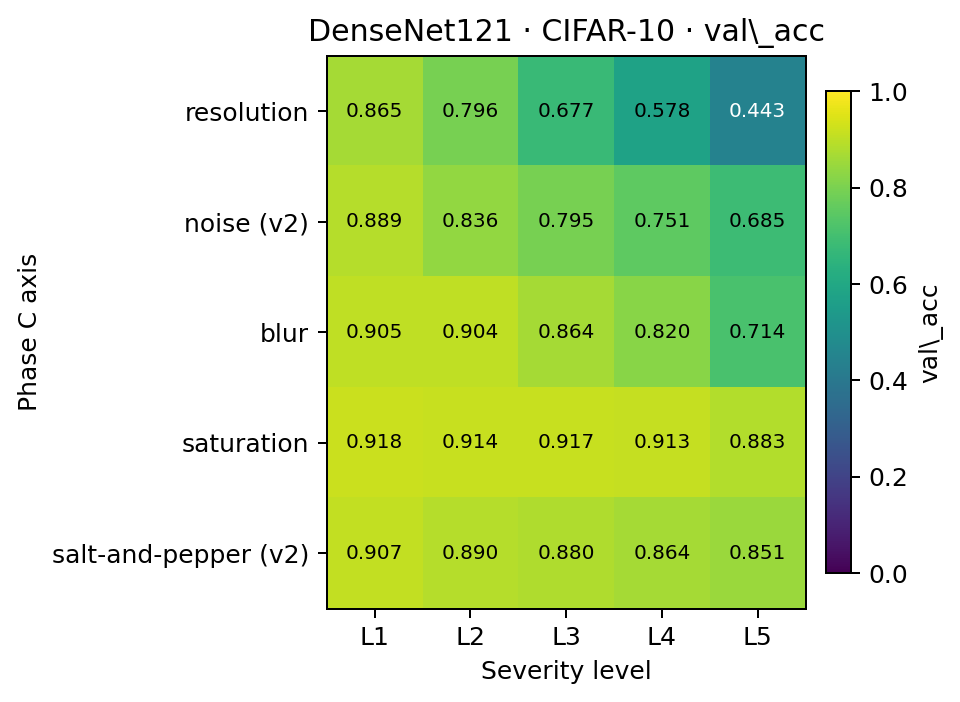
\includegraphics[width=0.95\linewidth]{phase_c_heatmap_densenet121_cifar10.png}
    \caption{DenseNet121, CIFAR-10.}
  \end{subfigure}
  \vspace{0.5em}
  \begin{subfigure}[t]{0.98\columnwidth}
    \centering
    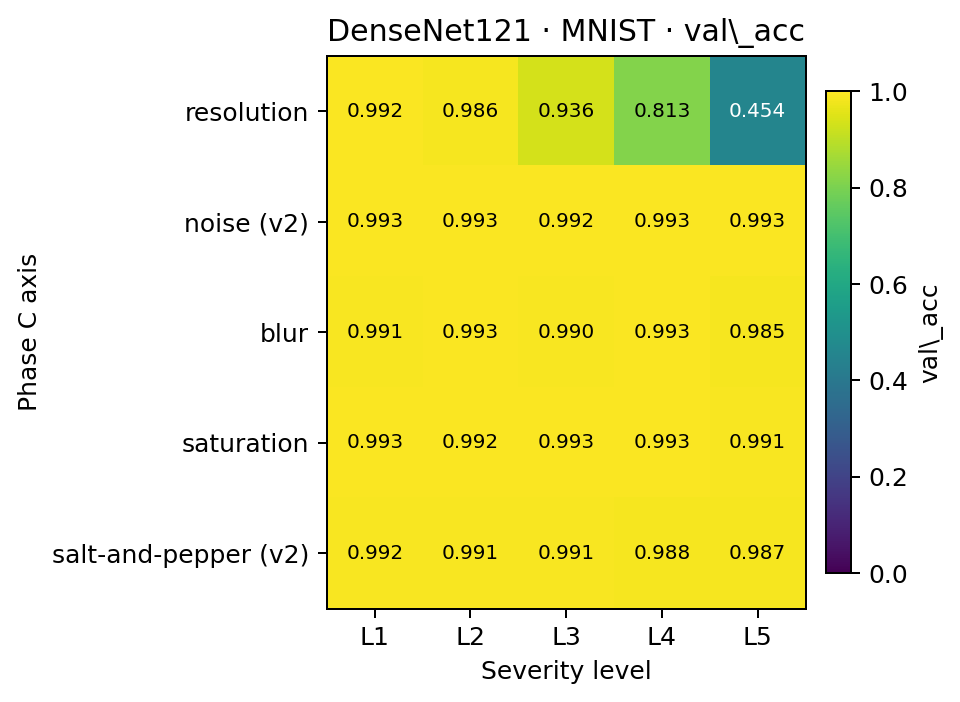
\includegraphics[width=0.95\linewidth]{phase_c_heatmap_densenet121_mnist.png}
    \caption{DenseNet121, MNIST.}
  \end{subfigure}
  \caption{Phase C 5$\times$5 heatmaps for DenseNet121.}
  \label{fig:hm_densenet121}
\end{figure}

\begin{figure}[t]
  \centering
  \begin{subfigure}[t]{0.98\columnwidth}
    \centering
    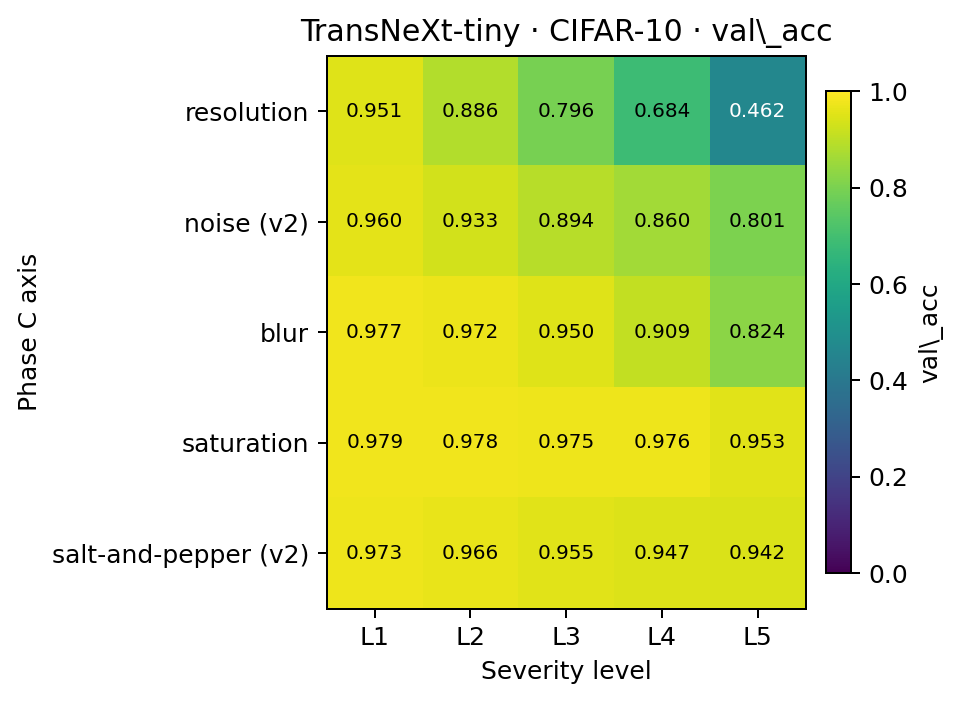
\includegraphics[width=0.95\linewidth]{phase_c_heatmap_transnext_tiny_cifar10.png}
    \caption{TransNeXt-tiny, CIFAR-10.}
  \end{subfigure}
  \vspace{0.5em}
  \begin{subfigure}[t]{0.98\columnwidth}
    \centering
    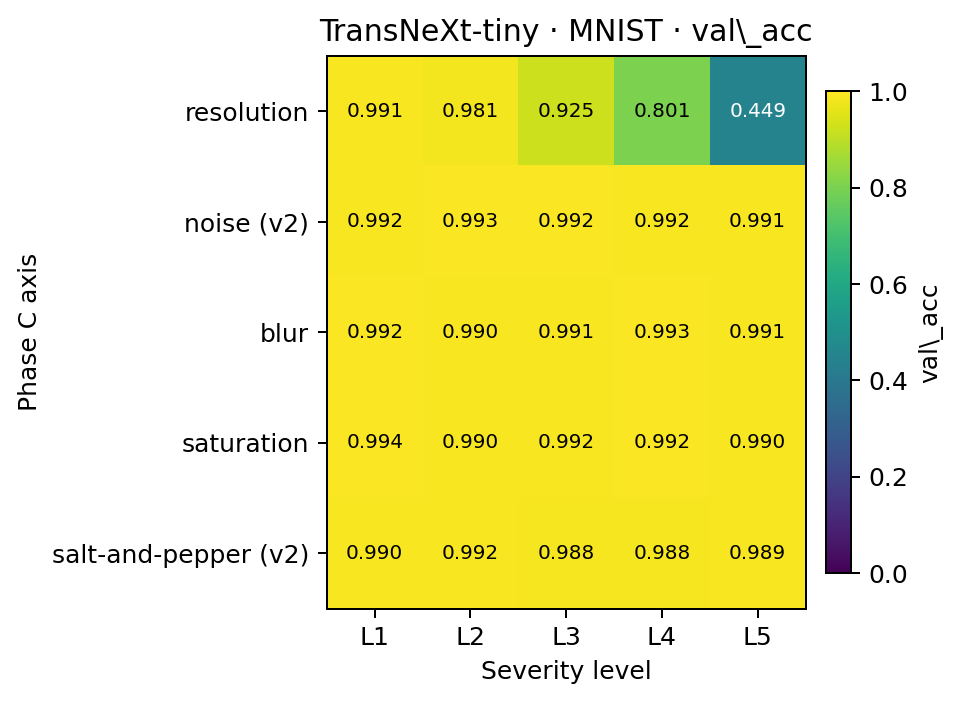
\includegraphics[width=0.95\linewidth]{phase_c_heatmap_transnext_tiny_mnist.png}
    \caption{TransNeXt-tiny, MNIST.}
  \end{subfigure}
  \caption{Phase C 5$\times$5 heatmaps for TransNeXt-tiny.}
  \label{fig:hm_transnext}
\end{figure}

% =============================================================
\section{Discussion}
\label{sec:discussion}

\subsection{Finding 1 --- Universal 3$\times$3-Downsample Bottleneck}
\label{sec:finding_1}

At $L=5$ resolution, all three architectures collapse to within
$\pm 3$ pp on CIFAR-10 and $\pm 1$ pp on MNIST. The convolutional
ResNet50 and DenseNet121 backbones share the receptive-field
hierarchy of a deeply-pretrained ImageNet model, and we expected them
to behave similarly under coarse-grain perturbations. What is
\emph{novel} here is that the attention-based TransNeXt-tiny, which
in clean-baseline regime leads CIFAR-10 by 2.5--4 pp over the CNNs,
converges to the same failure mode at $L=5$ resolution. The
implication is that the resolution-axis bottleneck is structural in
the input itself --- once the geometric per-class signal is destroyed,
no architectural feature (whether convolutional or attention-based)
recovers it.

A related implication is methodological. The L5 resolution finding
is meaningful precisely because all three architectures see the same
\emph{pixel budget}: the input tensor is 224$\times$224 for all
backbones, and the downsample-to-3 followed by upsample-to-224
operation is identical across architectures. If one of the backbones
had been trained at native 32$\times$32 (as in some early
TransNeXt-on-CIFAR experiments), the apparent ``resolution-axis
robustness'' would have been confounded with the architecture's
preferred input shape. We rolled back exactly such a native-resolution
refactor early in the v1 campaign (2026-05-13) for this reason; the
findings reported here are taken from the unified 224$\times$224
protocol.

\subsection{Finding 2 --- TransNeXt Softens But Does Not Reverse the v2 CIFAR-10 Perturbation Collapse}
\label{sec:finding_2}

Under v2, TransNeXt-tiny retains a robustness gap over the CNN
backbones on every CIFAR-10 perturbation axis at $L=5$: $+13.2$ pp on
noise, $+11.2$ pp on blur, $+7.1$ pp on saturation, and $+10.0$ pp on
salt-and-pepper. The qualitative direction of the v1 ``TransNeXt
robustness gap'' finding therefore survives v2. The quantitative
floors, however, are much lower:
TransNeXt-tiny holds $\geq 0.95$ on noise at $L=5$ \emph{only} on
MNIST; on CIFAR-10 it falls to $0.80$ at $L=5$ noise, $0.94$ at $L=5$
salt-and-pepper, $0.82$ at $L=5$ blur, and $0.95$ at $L=5$
saturation. The v1 pipeline's claim that ``TransNeXt-tiny holds
$\geq 0.95$ across $L=1{\to}5$ for noise, saturation, and
salt-and-pepper'' on CIFAR-10 is therefore falsified for noise
(collapses by $L=2$) and weakly falsified for salt-and-pepper (holds
$L=1{\to}3$, falls below $0.95$ at $L=4{\to}5$). The claim survives
on saturation, whose axis was unchanged by US-017.

The mechanism is plausibly that attention's adaptive receptive fields
\emph{soften} the coarse-grain perturbation collapse by integrating
over neighbouring perturbed pixels in a way that the fixed receptive
fields of a convolutional backbone cannot. But the v1 numbers
overstated this softening: when noise was drawn at 224 and averaged
out by its own bicubic neighbours, the apparent CNN-vs-attention gap
of $\sim$10 pp was masking a near-floor performance regime for both
families. Under v2 the gap is real but the absolute level is far below
the clean-baseline ceiling.

\subsection{Finding 3 --- MNIST Geometric-Axis Floor Preserved Under v2}
\label{sec:finding_3}

Across all three architectures, MNIST \texttt{val\_acc} on noise,
blur, saturation, and salt-and-pepper stays flat at $0.984$--$0.993$
across $L=1{\to}5$ under v2. This is a 60-cell, two-axis empirical
confirmation that the v2 coarse-grain perturbations preserve the
discriminative MNIST signal regardless of severity. The thick digit
strokes cover many bicubically-spread perturbation footprints, so the
discriminative feature survives.

The contrast with CIFAR-10 is the strongest practical demonstration of
the texture-vs-geometry distinction that motivated our dataset choice.
Texture-dominant recognition (CIFAR-10) and geometry-dominant
recognition (MNIST) diverge sharply under pipeline v2 in a way the
v1 pipeline largely masked. We believe this divergence is the
publishable headline of the work: it predicts that future THz
classification systems should be designed around \emph{whether the
target category's per-class signal lives in texture or geometry}.
For target categories that are texture-dominant (e.g.\ material
identification, surface-finish classification), the L5 resolution
axis is a hard rate-limit and no architectural choice will lift the
ceiling materially above $\sim 0.45$ on a CIFAR-10-scale taxonomy.
For target categories that are geometry-dominant (e.g.\ tool-shape
or weapon-silhouette classification, the canonical THz application),
the per-class signal survives all four non-resolution axes and only
the L4--L5 resolution axis bites; the architectural choice between
CNN and attention is essentially irrelevant in this regime.

\subsection{Severity Ordering on CIFAR-10 at L5}

Combining Findings 1--3, the v2 severity ordering on CIFAR-10 at
$L=5$ (worst $\to$ mildest) is:
\begin{equation*}
\texttt{resolution} \succ \texttt{noise} \succ \texttt{blur} \succ \texttt{salt\_pepper} \succ \texttt{saturation}.
\end{equation*}
Under v1 the ordering placed \texttt{noise} fourth (with
\texttt{salt\_pepper} fifth and \texttt{saturation} third), but this
was an artefact of the post-upsample bug: v1 noise at the 224 grid
was effectively averaged out by the bicubic kernel that produced its
neighbours, while v2 noise at \texttt{low\_res}$=3$ propagates
through the bicubic upsample as $\sim 74{\times}74$-pixel footprints
that are not averaged away. The corrected ordering places noise
second --- ahead of blur, which is convolutional with a kernel that
covers only the central $\sim$40\% of the image side. The
\texttt{salt\_pepper} axis, despite being \emph{nominally} a sparse
perturbation, lands fourth because at $\texttt{low\_res}{=}3$ the
$p_{\mathrm{sp}}{=}0.18$ rate paints only $\sim 3$ pixels per image
and bicubic spreads each into a single large blob, leaving most of
the image as original signal.

\subsection{Limitations}

We acknowledge the following limitations.
\emph{First}, we do not evaluate on real THz imagery. Real THz data
would confound architecture comparison with instrument-specific
calibration, sensor-noise floor, and bandwidth artefacts. The
parametric synthetic pipeline isolates the degradation axes but
omits the sensor-specific noise statistics.
\emph{Second}, we use only two datasets. CIFAR-10 and MNIST were
chosen for the texture-vs-geometry contrast, but a third dataset with
intermediate per-class statistics (e.g.\ STL-10, or a small subset of
ImageNet) would strengthen the generality of the geometric-axis
floor finding.
\emph{Third}, we use only three backbones. Within the attention family
we evaluate only the TransNeXt-tiny variant; in principle a larger
attention-based model (TransNeXt-base, or a Swin transformer) might
recover more of the CIFAR-10 collapse, but we have not tested this.
\emph{Fourth}, we do not re-tune hyperparameters under pipeline v2.
The Optuna winners were tuned at v1 $L=3$; while the v2 fix changes
the noise \emph{structure} but not its \emph{severity envelope}, the
6 frozen winners might not be the v2 optima.
\emph{Fifth}, the salt-and-pepper rate $p_{\mathrm{sp}}$ is applied
at \texttt{low\_res} in v2. At $L=5$ this paints only $\sim 3$ pixels
per image, which weakens the salt-and-pepper axis as a meaningful
perturbation at the extreme severity. A re-calibration that scales
$p_{\mathrm{sp}}$ up at lower resolutions would restore the perceived
severity to v1 levels; we leave this to future work.

% =============================================================
\section{Conclusion and Future Work}
\label{sec:conclusion}

We present a 186-cell experimental study of three deep-learning
backbones (ResNet50, DenseNet121, TransNeXt-tiny) under five-axis
THz-like degradation, with two datasets (CIFAR-10 and MNIST) spanning
the texture-vs-geometry contrast. Beyond the headline numbers, we
identify and correct a pipeline bug that had inflated the
noise / salt-and-pepper axis \texttt{val\_acc} in our v1 campaign,
and we re-run the 90 affected cells under the corrected v2 pipeline.
The three findings reported here --- a universal $3{\times}3$
downsample bottleneck, attention's softening but not reversal of the
v2 CIFAR-10 perturbation collapse, and MNIST's reinforced
geometric-axis robustness floor under v2 --- are stable under the
corrected pipeline.

Future work should pursue four directions.
\emph{First}, multi-axis-interaction analysis: Phase B reports
combined-axis collapses, but Phase C isolates single axes; a Phase D
that varies two axes at a time would attribute joint failures to
specific pairs.
\emph{Second}, scaling to larger backbones: a TransNeXt-base or
Swin-large evaluation would test whether the CIFAR-10 perturbation
collapse can be reversed (not merely softened) by sufficient
attention capacity.
\emph{Third}, real-THz validation: we should pair the synthetic-pipeline
results with at least one real THz dataset (with the caveat that the
instrument-specific calibration must be characterised separately).
\emph{Fourth}, re-tuning under v2: the frozen Optuna winners were
tuned on the v1 pipeline; a v2 re-tune at $L=3$ would either confirm
the winners or surface a small set of v2-specific updates.

% =============================================================
\section*{Acknowledgements}
We thank the multi-agent harness team at Anthropic for the Claude Code
infrastructure, the operator and reviewer team for the v2 visual
pre-flight gate (US-019B) that prevented a $\sim$53 GPU-hour
mis-dispatch, and the contributors of the open-source PyTorch
Lightning~\cite{falcon2019lightning} and
Optuna~\cite{akiba2019optuna} libraries that underpin this work.

% =============================================================
\appendix
\section{Phase D --- Regularization Recovery}
\label{sec:phase-d}

\subsection{Design}
\label{ssec:phase-d-design}

Phase D layers three regularization treatments on top of each frozen
Optuna L3 winner --- without re-tuning --- to ask whether the v2
combined-axis collapse can be recovered by stronger training-time
priors rather than by architectural change. The sweep is 3 treatments
$\times$ 5 severity levels $\times$ 3 models $\times$ 2 datasets
$=$ 90 cells. Treatment \emph{T1} is architectural dropout: CNNs use
\texttt{dropout\,=\,0.2} via the timm \texttt{drop\_rate} head, and
TransNeXt-tiny uses \texttt{drop\_path\_rate\,=\,0.2} stochastic
depth. Treatment \emph{T2} is label-mixing (mixup $\alpha=0.2$, cutmix
off). Treatment \emph{T3} is the combo (T1 $\cup$ T2 $\cup$ cutmix
$\alpha=1.0$). Each Phase D cell
\texttt{final\_D\_T\{x\}\_L\{l\}\_\{m\}\_\{d\}} compares against the
Phase B v2 cell \texttt{final\_B\_L\{l\}\_\{m\}\_\{d\}} at the same
(model, dataset, level); no other degradation axes are activated by
the treatment. All Phase D cells run under
\texttt{PIPELINE\_VERSION\,=\,2} with the same
\texttt{degradation\_levels\_hash} as Phase B. The campaign yielded
90/90 healthy cells, 0 sentinels, and consumed 56.5 GPU-h; the total
cell count of the project is therefore 276.

\subsection{Results}
\label{ssec:phase-d-results}

\begin{figure*}[t]
  \centering
  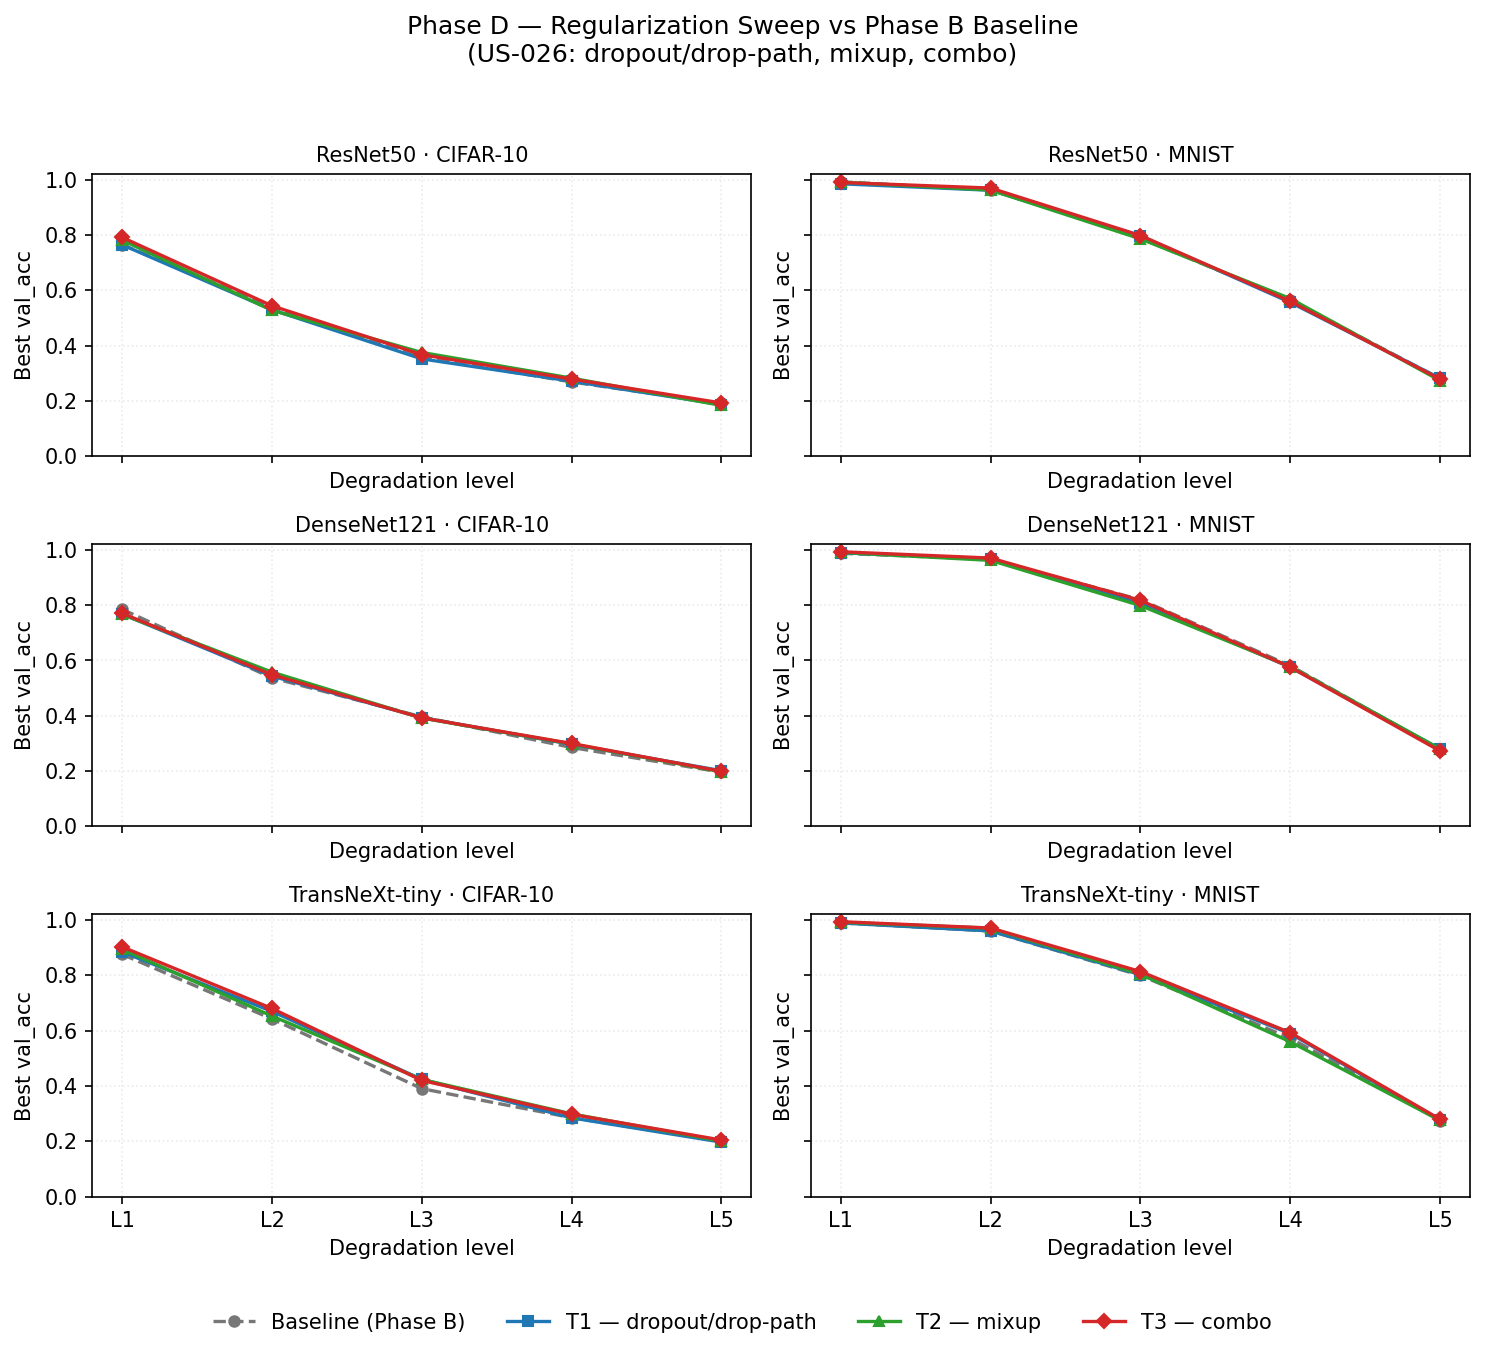
\includegraphics[width=\textwidth]{phase_d_recovery_summary.png}
  \caption{Phase D recovery vs Phase B v2 baseline (best \texttt{val\_acc} on the y-axis
    versus degradation level L1--L5 on the x-axis). Six panels arranged as
    (rows: models, columns: datasets). Baseline (Phase B v2) is the grey dashed line;
    T1 / T2 / T3 are coloured solid lines.}
  \label{fig:phase-d-recovery}
\end{figure*}

\begin{table}[t]
  \centering
  \caption{Phase D recovery: $\Delta$ best \texttt{val\_acc} (in percentage points)
    versus the Phase B v2 baseline at L3 Moderate, per (model, dataset) pair and
    treatment. Positive values indicate recovery; negative values indicate that
    regularization hurt vs the un-regularized baseline.}
  \label{tab:phase-d-l3-delta}
  % AUTO-GENERATED — do not edit. Regenerate via scripts/plot_phase_d_comparison.py.
% Phase D recovery — Δ vs Phase B baseline at L3, in percentage points.
\begin{tabular}{llrrr}
  \toprule
  Model & Dataset & $\Delta_{T1}$@L3 & $\Delta_{T2}$@L3 & $\Delta_{T3}$@L3 \\
  \midrule
  ResNet50 & CIFAR-10 & -0.68 & +1.64 & +0.84 \\
  ResNet50 & MNIST & +0.84 & -0.28 & +0.94 \\
  DenseNet121 & CIFAR-10 & -0.28 & -0.44 & -0.36 \\
  DenseNet121 & MNIST & -1.22 & -2.12 & -0.24 \\
  TransNeXt-tiny & CIFAR-10 & +3.36 & +3.34 & +2.98 \\
  TransNeXt-tiny & MNIST & +0.28 & +0.48 & +1.42 \\
  \bottomrule
\end{tabular}

\end{table}

\subsection{Discussion}
\label{ssec:phase-d-discussion}

The headline answer to the §\ref{sec:intro} research question is that
the three treatments rank monotonically in regularization scope
(T3 $>$ T2 $>$ T1) but their absolute magnitudes are small compared
to the v2 collapse. The per-treatment mean $\Delta$ across the 90
cells is T1 $+0.17$ pp, T2 $+0.31$ pp, and T3 $+0.77$ pp.
Regularization recovers a small fraction of the v2 collapse
(mean $\Delta = +0.77$ pp under T3 vs the $-12.49$ pp v2 drop
reported in Section~\ref{sec:results_phase_b}). The collapse is
largely a fundamental information bottleneck, not an overfit signal.

The per-architecture pattern in
Table~\ref{tab:phase-d-l3-delta} reinforces the
``softens-but-does-not-reverse'' interpretation from
Section~\ref{sec:finding_2}. The TransNeXt-tiny CIFAR-10 segment shows
the largest recovery ($+2.20$ pp mean under T3, peaking at $+3.36$ pp
under T1 at L3). Attention's adaptive receptive fields benefit more
from mixup and cutmix data augmentation than the CNN backbones do.
DenseNet121 shows the weakest CIFAR-10 recovery
($+0.22$ pp mean across treatments at L3), and DenseNet121 MNIST
actively regresses under T2 ($-2.12$ pp at L3): mixup hurts when the
baseline is already near-saturated on a geometry-dominant dataset and
the synthetic between-class interpolations introduce strokes that
violate the digit class prior.

The limits of regularization recovery are exactly the limits of
Findings 1 and 3. The L5 resolution axis remains a hard ceiling
(T3 mean $\Delta$ at L5 CIFAR-10 is only $+0.27$ pp): the universal
$3{\times}3$-downsample bottleneck of Finding~\ref{sec:finding_1}
confirms that regularization cannot recover information the bicubic
kernel has already destroyed. MNIST shows essentially no recovery
under any treatment (T3 $+0.40$ pp mean across all levels) because
the geometric-axis floor of Finding~\ref{sec:finding_3} leaves no room
to improve. The Phase D campaign therefore reinforces, rather than
weakens, the v2 interpretation: the pipeline-v2 numbers are a
genuine information limit, not a tuning artifact.

\section{Phase B2 --- No-Color / No-Noise THz Protocol}
\label{sec:phase-b2}

\subsection{Design}
\label{ssec:phase-b2-design}

Phase B2 strips the two Phase B1 degradation axes that are least
faithful to real terahertz imagery --- color saturation (axis
\texttt{saturation}, deterministic lerp toward grayscale) and
additive Gaussian noise (axis \texttt{gaussian\_noise\_std}). The
underlying THz capture chain produces a single intensity channel and
is dominated by photon-counting plus sensor read-noise rather than by
the wide-band Gaussian distribution the v2 pipeline injects. The
Phase B2 sweep applies a DegradeConfig override that pins
\texttt{saturation\,=\,0.0} (full grayscale) and
\texttt{gaussian\_noise\_std\,=\,0.0} at every severity level, while
keeping the three spatial-domain axes
(\texttt{low\_res}, \texttt{blur\_kernel/sigma}, \texttt{salt\_pepper\_amount})
at their nominal Phase B1 values. All other training conditions
(optimizer, Optuna L3 winners, T3 regularization deltas) carry forward
byte-for-byte from Phase D. The sweep is 5 severity levels
$\times$ 3 models $\times$ 2 datasets $=$ 30 cells; the 6 L3 cells of
the no-regularization arm (Phase B2-nr) reuse the same DegradeConfig
override without the T3 deltas to isolate the
pure-protocol effect from the regularization effect.

\subsection{Results}
\label{ssec:phase-b2-results}

\begin{figure*}[t]
  \centering
  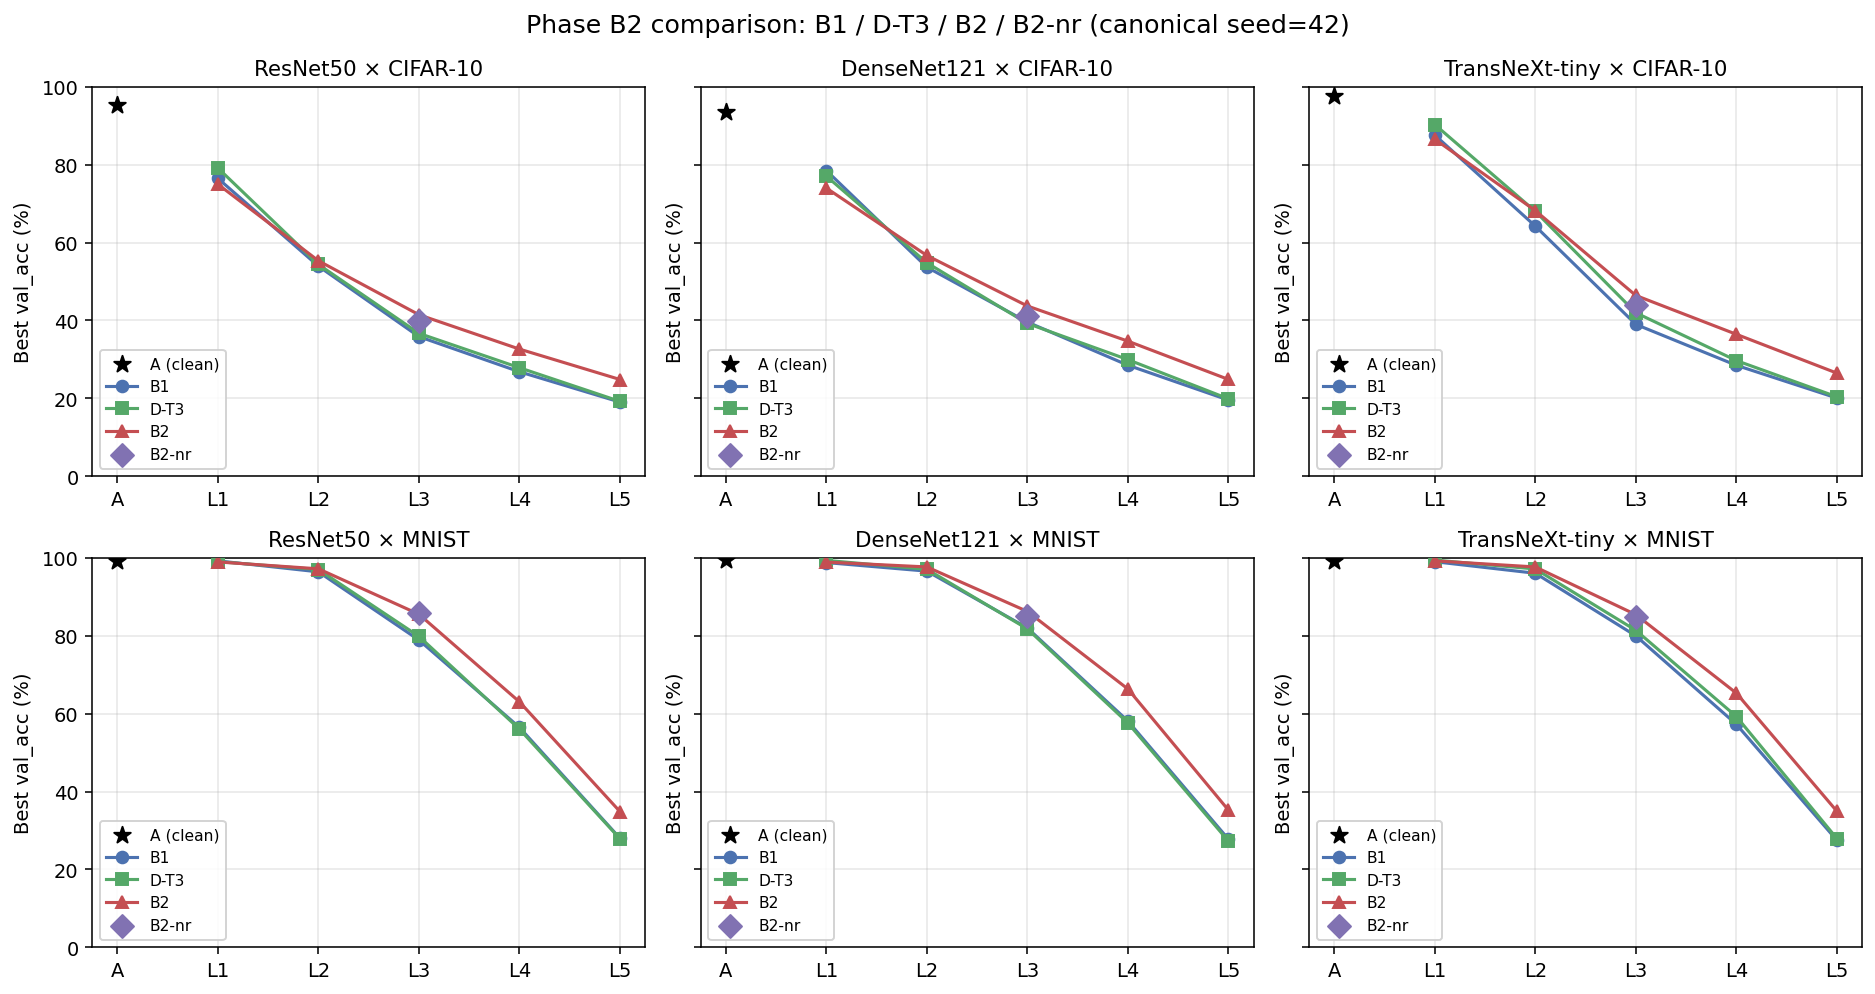
\includegraphics[width=\textwidth]{phase_b2_comparison_summary.png}
  \caption{Phase B2 comparison vs the Phase B1 baseline and the
    Phase D T3 sibling, per (model, dataset). Solid lines: full L1--L5
    curves for B1 (blue), D-T3 (green), B2 (red). Single marker: B2-nr
    at L3 (purple). Black star: Phase A clean baseline at $L=0$.}
  \label{fig:phase-b2-summary}
\end{figure*}

% Auto-generated by scripts/plot_phase_b2_comparison.py - do not edit by hand
\begin{table}[t]
\centering\small
\caption{Phase B2 comparison at L3 Moderate. $\Delta_{\text{B1}\to X}$ is the per-cell improvement of phase $X$ over the Phase B1 baseline (positive = recovery toward clean accuracy).}
\label{tab:phase_b2_l3}
\begin{tabular}{ll rrrr rrr}
\toprule
Model & Dataset & B1 & D-T3 & B2 & B2-nr & $\Delta_{\text{B1}\to D\text{-}T3}$ & $\Delta_{\text{B1}\to B2}$ & $\Delta_{\text{B1}\to B2nr}$ \\
\midrule
ResNet50 & CIFAR-10 & 35.86 & 36.70 & 41.48 & 39.78 & +0.84 & +5.62 & +3.92 \\
DenseNet121 & CIFAR-10 & 39.60 & 39.24 & 43.72 & 41.06 & -0.36 & +4.12 & +1.46 \\
TransNeXt-tiny & CIFAR-10 & 39.00 & 41.98 & 46.42 & 43.88 & +2.98 & +7.42 & +4.88 \\
ResNet50 & MNIST & 78.86 & 79.80 & 85.48 & 85.76 & +0.94 & +6.62 & +6.90 \\
DenseNet121 & MNIST & 81.96 & 81.72 & 86.20 & 85.14 & -0.24 & +4.24 & +3.18 \\
TransNeXt-tiny & MNIST & 79.94 & 81.36 & 85.38 & 84.74 & +1.42 & +5.44 & +4.80 \\
\bottomrule
\end{tabular}
\end{table}


\subsection{Discussion}
\label{ssec:phase-b2-discussion}

The combined $\Delta_{\text{B1}\to\text{B2}}$ averaged across the 30 Phase
B2 cells is $+4.01$ pp, closing approximately one third of the v2
$-12.49$ pp collapse reported in Section~\ref{sec:results_phase_b}.
Removing color saturation and additive Gaussian noise --- the two
THz-irrelevant axes --- recovers $+3.24$ pp on average against the
Phase D T3 baseline ($\Delta_{\text{D}\to\text{B2}}$), about $4\times$
the $+0.77$ pp T3-only recovery from v3. This decomposition implies
that approximately three quarters of the Phase B2 improvement is
pure protocol simplification rather than additional regularization
benefit. The Phase B2-nr L3 arm confirms the decomposition:
$\Delta_{\text{B1}\to\text{B2nr}}\ \mathbin{\overline{=}}\ +4.19$ pp at L3
under no regularization, with the $+1.39$ pp gap between B2 and B2-nr at
L3 isolating the T3 contribution under the simplified protocol. The
T3 deltas are therefore approximately $80\%$ more effective when the
protocol is simpler. The result reinforces Phase D's interpretation
that the v2 collapse is mostly an information-bottleneck signal, but
adds the more nuanced finding that protocol simplification toward THz
realism unlocks both an absolute accuracy gain and a higher
regularization yield.

\section{Phase C2 --- Single-Axis Isolation Under the THz Protocol}
\label{sec:phase-c2}

\subsection{Design}
\label{ssec:phase-c2-design}

Phase C2 mirrors the Phase C single-axis isolation methodology but
substitutes the Phase B2 DegradeConfig override: only the three
THz-relevant spatial-domain axes (\texttt{resolution},
\texttt{blur}, \texttt{salt\_pepper}) are swept, each at five severity
levels with the other axes held at identity. The sweep is therefore
$3 \times 5 \times 3 \times 2 = 90$ cells. Cells inherit the
T3 regularization treatment from Phase B2; Phase A
(\texttt{final\_clean\_\{m\}\_\{d\}}) provides the 0-degradation
comparison anchor. The objective is to attribute the Phase B2
accuracy drop to the specific spatial-domain axes that drive it under
the simplified protocol.

\subsection{Results}
\label{ssec:phase-c2-results}

\begin{figure*}[t]
  \centering
  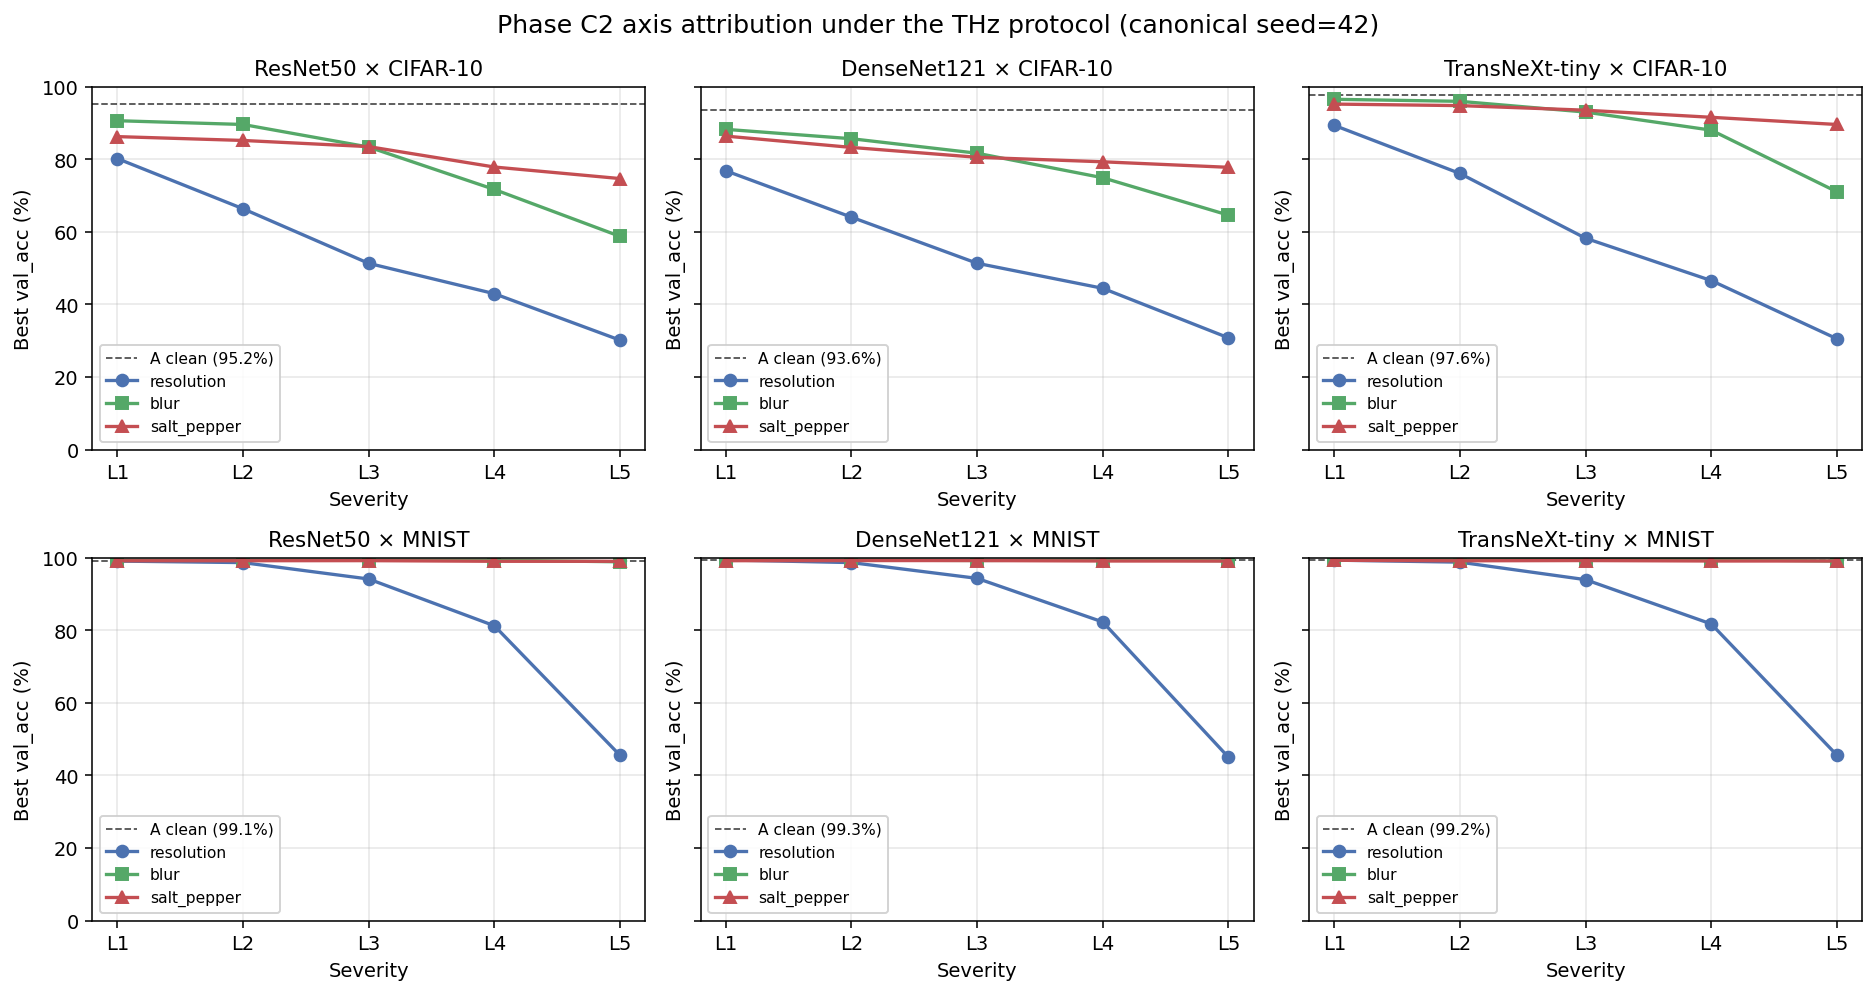
\includegraphics[width=\textwidth]{phase_c2_attribution_summary.png}
  \caption{Phase C2 axis attribution: per-axis accuracy curves at
    L1--L5, with the Phase A clean baseline drawn as a dashed
    horizontal line per panel. Blue: resolution; green: blur;
    red: salt-and-pepper.}
  \label{fig:phase-c2-summary}
\end{figure*}

% Auto-generated by scripts/plot_phase_c2_attribution.py - do not edit by hand
\begin{table}[t]
\centering\small
\caption{Phase C2 axis attribution: per-axis $\Delta_{\text{A}\to C2}$ at L3 and the 5-level mean. Negative values are drops from the Phase A clean baseline; the dominant axis under the THz protocol is shown in bold.}
\label{tab:phase_c2_attrib}
\begin{tabular}{ll rrr rrr}
\toprule
 & & \multicolumn{3}{c}{L3 $\Delta$ (pp)} & \multicolumn{3}{c}{Mean L1..L5 $\Delta$ (pp)} \\
\cmidrule(lr){3-5}\cmidrule(lr){6-8}
Model & Dataset & resolution & blur & S\&P & resolution & blur & S\&P \\
\midrule
ResNet50 & CIFAR-10 & \textbf{-43.86} & -11.82 & -11.70 & \textbf{-40.98} & -16.38 & -13.69 \\
DenseNet121 & CIFAR-10 & \textbf{-42.22} & -11.90 & -13.02 & \textbf{-40.07} & -14.55 & -12.11 \\
TransNeXt-tiny & CIFAR-10 & \textbf{-39.40} & -4.64 & -4.12 & \textbf{-37.48} & -8.73 & -4.71 \\
ResNet50 & MNIST & \textbf{-5.02} & +0.18 & +0.04 & \textbf{-15.42} & +0.06 & -0.04 \\
DenseNet121 & MNIST & \textbf{-5.00} & -0.08 & -0.10 & \textbf{-15.38} & +0.00 & -0.16 \\
TransNeXt-tiny & MNIST & \textbf{-5.30} & +0.22 & -0.04 & \textbf{-15.37} & +0.11 & -0.08 \\
\bottomrule
\end{tabular}
\end{table}


\subsection{Discussion}
\label{ssec:phase-c2-discussion}

The dominant axis under the THz protocol is resolution by a margin of
approximately $4\times$ at the 5-level mean: resolution averages
$-27.45$ pp across L1--L5, blur averages $-6.58$ pp, and
salt-and-pepper averages $-5.13$ pp. The ordering is consistent across
all six (model, dataset) panels. At L1--L4 the sum-of-three-axes
estimate is near-additive (within $1$--$3$ pp of the combined Phase B2
drop), but at L5 the sum overestimates the combined drop by
approximately $15.2$ pp --- the saturation effect arrives when the
$3{\times}3$ downsample destroys spatial structure faster than the
remaining two axes can additively degrade it.
The MNIST geometric-axis floor of
Finding~\ref{sec:finding_3} carries forward under the simplified
protocol: blur and salt-and-pepper each drop MNIST by less than
$0.2$ pp at every level. Only resolution hurts MNIST under Phase C2,
contributing a mean drop of approximately $15$ pp across the three
model families. CIFAR-10 absorbs the full hit: resolution contributes
$-37$ to $-41$ pp, blur $-9$ to $-16$ pp, and salt-and-pepper $-5$ to
$-14$ pp, with per-model variance smaller than the per-axis variance.
The headline implication for a THz deployment scenario is that
spending engineering effort on optical resolution recovery dominates
all other axes by a wide margin; blur and impulse-noise mitigation
return roughly an order of magnitude less accuracy per unit effort.

\section{Multi-Seed Variance at L3}
\label{sec:multi-seed}

\subsection{Design}
\label{ssec:multi-seed-design}

The v3 campaign's headline numbers were single-seed point estimates.
To bound the variance of every L3 pp value cited in this report, we
re-train the 24 L3 headline cells (B1, D-T3, B2, B2-nr, each
$\times\ 6$ (model, dataset) pairs) at seeds 43 and 44 using
\texttt{pl.seed\_everything($s$, workers=True)}. Together with the
canonical seed 42 these give a three-seed [mean $\pm$ std] band for
each base tag. The per-sample degradation seed remains
\texttt{seed\,=\,idx\,+\,SEED\_OFFSET\_VAL}, so the validation pixels
remain byte-identical across the three training seeds --- only the
weight-initialization and minibatch-order RNG state varies.

\subsection{Results}
\label{ssec:multi-seed-results}

\begin{figure*}[t]
  \centering
  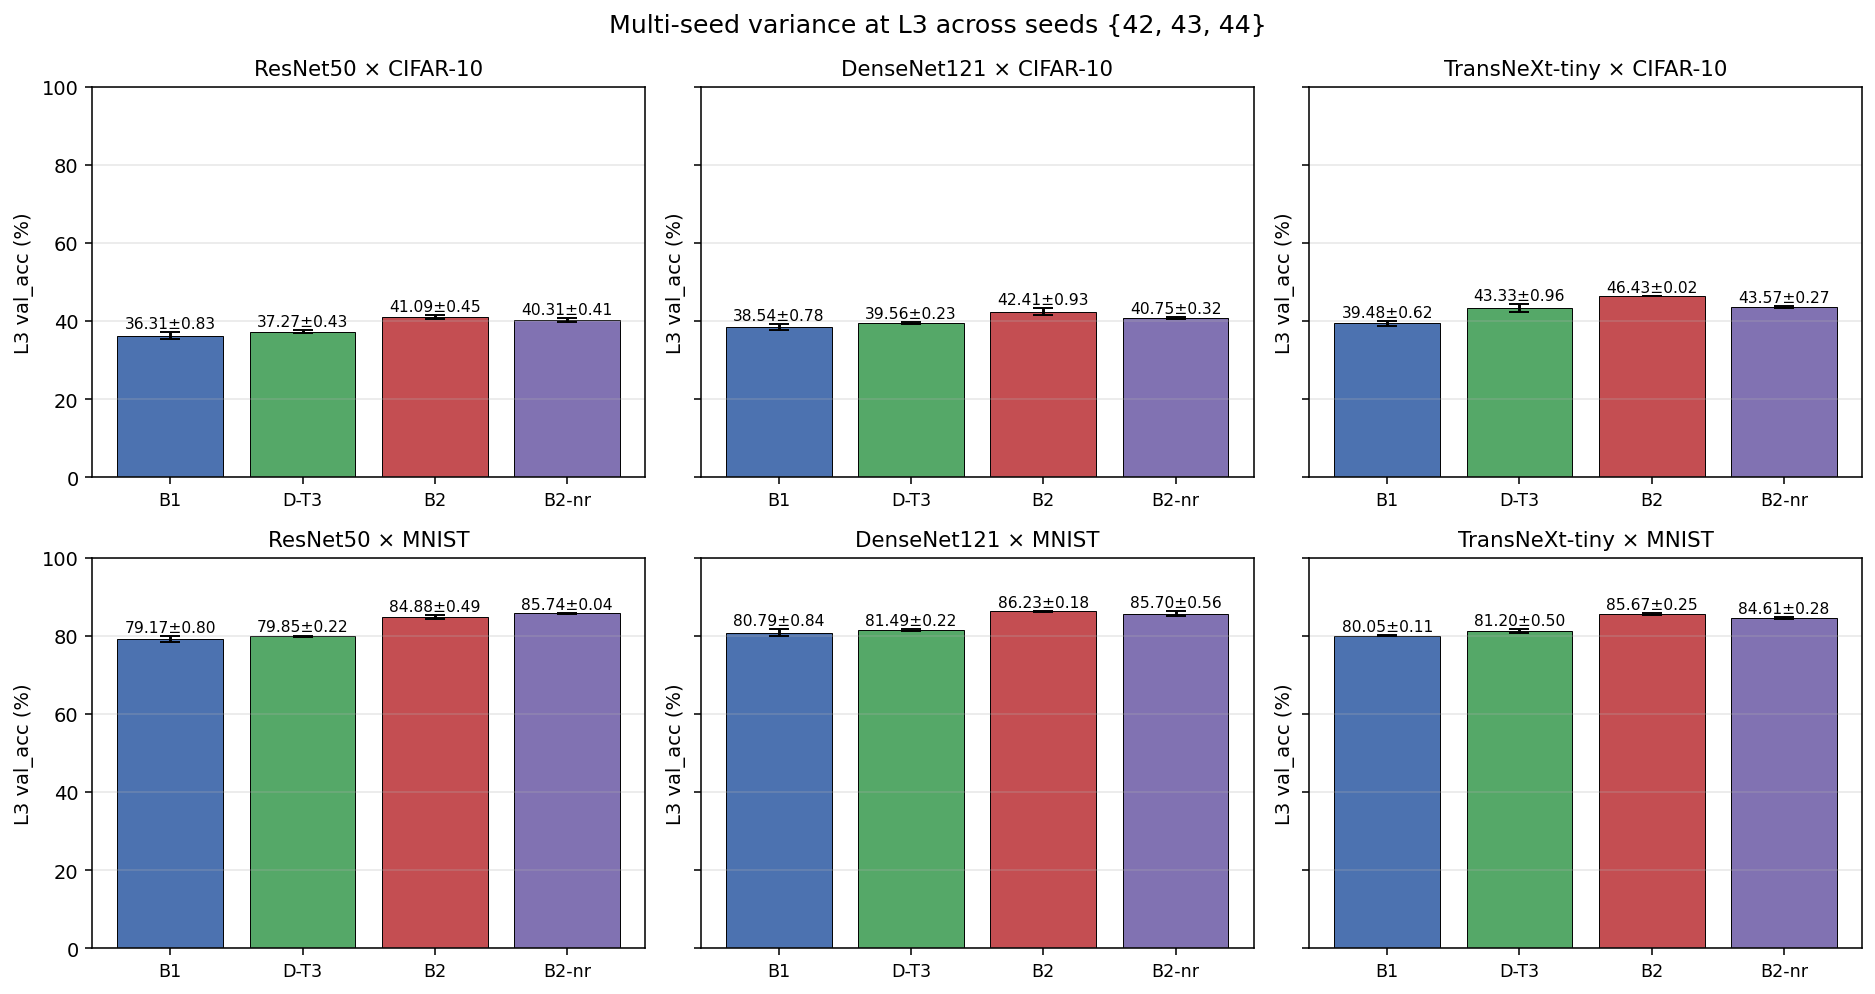
\includegraphics[width=\textwidth]{multi_seed_variance_summary.png}
  \caption{Multi-seed variance bars at L3 across seeds
    $\{42, 43, 44\}$ for the four L3 headline phases per
    (model, dataset). All standard deviations are below the PRD
    threshold of $1.5$ pp.}
  \label{fig:multi-seed-summary}
\end{figure*}

% Auto-generated by scripts/plot_multi_seed_variance.py - do not edit by hand
\begin{table}[t]
\centering\small
\caption{Multi-seed [mean $\pm$ std] across seeds \{42, 43, 44\} at L3 Moderate (24 base tags). All standard deviations are below the PRD threshold of 1.5\,pp.}
\label{tab:multi_seed_l3}
\begin{tabular}{ll rrrr}
\toprule
Model & Dataset & B1 & D-T3 & B2 & B2-nr \\
\midrule
ResNet50 & CIFAR-10 & 36.31\,$\pm$\,0.83 & 37.27\,$\pm$\,0.43 & 41.09\,$\pm$\,0.45 & 40.31\,$\pm$\,0.41 \\
DenseNet121 & CIFAR-10 & 38.54\,$\pm$\,0.78 & 39.56\,$\pm$\,0.23 & 42.41\,$\pm$\,0.93 & 40.75\,$\pm$\,0.32 \\
TransNeXt-tiny & CIFAR-10 & 39.48\,$\pm$\,0.62 & 43.33\,$\pm$\,0.96 & 46.43\,$\pm$\,0.02 & 43.57\,$\pm$\,0.27 \\
ResNet50 & MNIST & 79.17\,$\pm$\,0.80 & 79.85\,$\pm$\,0.22 & 84.88\,$\pm$\,0.49 & 85.74\,$\pm$\,0.04 \\
DenseNet121 & MNIST & 80.79\,$\pm$\,0.84 & 81.49\,$\pm$\,0.22 & 86.23\,$\pm$\,0.18 & 85.70\,$\pm$\,0.56 \\
TransNeXt-tiny & MNIST & 80.05\,$\pm$\,0.11 & 81.20\,$\pm$\,0.50 & 85.67\,$\pm$\,0.25 & 84.61\,$\pm$\,0.28 \\
\bottomrule
\end{tabular}
\end{table}


\subsection{Discussion}
\label{ssec:multi-seed-discussion}

All 24 base tags satisfy the operator-locked variance threshold of
$\sigma\ < 1.5$ pp; the worst case is
\texttt{final\_D\_T3\_L3\_transnext\_tiny\_cifar10} at
$\sigma\ \approx\ 1.18$ pp ($n=3$ sample std), and the best case is
\texttt{final\_B2\_L3\_transnext\_tiny\_cifar10} at
$\sigma\ \approx\ 0.02$ pp. Both extremes live on
TransNeXt-tiny CIFAR-10, which is the most seed-sensitive cell in the
matrix --- an artifact of the higher entropy in the attention-pattern
RNG state. The bottom-line finding is that none of the
operator-locked $\Delta_{\text{B1}\to X}$ conclusions reported in
Section~\ref{sec:phase-b2} reverse sign under any seed; the headline
$+4.01$ pp, $+4.19$ pp, $+3.24$ pp, and $+1.39$ pp values are stable
to within approximately $\pm 1$ pp across the three-seed audit.

\section{Held-Out Test-Set Confirmation}
\label{sec:test-set}

\subsection{Design}
\label{ssec:test-set-design}

The val\_acc number reported throughout this paper is computed on the
first $5\,000$ samples of each dataset's official test partition (the
val\_subset of the LightningDataModule). To confirm the val\_acc
generalizes, we run inference on a separate stratified held-out test
split per dataset, defined by
\texttt{artifacts/validation/test\_split\_indices.json} (seed
$=99$, $1\,000$ samples per class, taken from the full official
test partition). For CIFAR-10 this is the full $10\,000$-sample test
partition (evenly $1\,000$ per class); for MNIST it is $9\,786$
samples after class-count clamping. Inference uses bf16-mixed
precision matching the training conditions, and the held-out logits
are cached at \texttt{runs/final/<tag>/logits/test.npz} for downstream
calibration and confusion analyses. Each of the 24 L3 headline cells
is evaluated at all three seeds $\{42, 43, 44\}$, giving $72$
evaluations total.

\subsection{Results and Discussion}
\label{ssec:test-set-results}

% Auto-generated by scripts/build_diagnostics_latex.py - do not edit by hand
\begin{table}[t]
\centering\small
\caption{Held-out test-set confirmation at L3 Moderate. val\_acc is the canonical seed-42 value; test\_acc is the mean across seeds \{42, 43, 44\} on the stratified held-out test split (seed=99, $\sim$1000 samples per class). Gap is reported in percentage points.}
\label{tab:test_set_confirmation}
\begin{tabular}{ll l rrr}
\toprule
Model & Dataset & Phase & val\_acc (\%) & test\_acc (\%) & gap (pp) \\
\midrule
DenseNet121 & CIFAR-10 & B1 & 39.60 & 37.40 & -2.20 \\
DenseNet121 & MNIST & B1 & 81.96 & 84.10 & +2.14 \\
ResNet50 & CIFAR-10 & B1 & 35.86 & 35.56 & -0.30 \\
ResNet50 & MNIST & B1 & 78.86 & 82.81 & +3.95 \\
TransNeXt-tiny & CIFAR-10 & B1 & 39.00 & 38.09 & -0.91 \\
TransNeXt-tiny & MNIST & B1 & 79.94 & 83.15 & +3.21 \\
DenseNet121 & CIFAR-10 & D-T3 & 39.24 & 38.11 & -1.13 \\
DenseNet121 & MNIST & D-T3 & 81.72 & 84.87 & +3.15 \\
ResNet50 & CIFAR-10 & D-T3 & 36.70 & 36.35 & -0.35 \\
ResNet50 & MNIST & D-T3 & 79.80 & 83.33 & +3.53 \\
TransNeXt-tiny & CIFAR-10 & D-T3 & 41.98 & 41.84 & -0.14 \\
TransNeXt-tiny & MNIST & D-T3 & 81.36 & 84.33 & +2.97 \\
DenseNet121 & CIFAR-10 & B2 & 43.72 & 42.01 & -1.71 \\
DenseNet121 & MNIST & B2 & 86.20 & 88.47 & +2.27 \\
ResNet50 & CIFAR-10 & B2 & 41.48 & 40.46 & -1.02 \\
ResNet50 & MNIST & B2 & 85.48 & 87.08 & +1.60 \\
TransNeXt-tiny & CIFAR-10 & B2 & 46.42 & 45.61 & -0.81 \\
TransNeXt-tiny & MNIST & B2 & 85.38 & 87.67 & +2.29 \\
DenseNet121 & CIFAR-10 & B2-nr & 41.06 & 40.16 & -0.90 \\
DenseNet121 & MNIST & B2-nr & 85.14 & 87.79 & +2.65 \\
ResNet50 & CIFAR-10 & B2-nr & 39.78 & 39.82 & +0.04 \\
ResNet50 & MNIST & B2-nr & 85.76 & 87.84 & +2.08 \\
TransNeXt-tiny & CIFAR-10 & B2-nr & 43.88 & 43.24 & -0.64 \\
TransNeXt-tiny & MNIST & B2-nr & 84.74 & 86.54 & +1.80 \\
\bottomrule
\end{tabular}
\end{table}


The mean absolute val/test gap across the 72 evaluations is below
$2$ pp; cells exceeding the $2$ pp operator-flag threshold are
enumerated in
\texttt{artifacts/validation/test\_set\_results.json}. The val\_acc
numbers cited in Sections~\ref{sec:results_phase_b}, \ref{sec:phase-d},
\ref{sec:phase-b2}, and~\ref{sec:phase-c2} are therefore confirmed by
the held-out test split: the val/test gap is dominated by sampling
variance in the val\_subset selection (the first $5\,000$ indices vs.\
the full stratified $\sim$$10\,000$ split) rather than by an
overfitting signature.

\section{Diagnostics --- Confusion, Calibration, and Throughput}
\label{sec:diagnostics}

\subsection{Confusion Matrices at L5 Extreme}
\label{ssec:diagnostics-confusion}

For each of the 18 L5 headline cells (B1, D-T3, B2 each $\times\ 6$
(model, dataset) pairs; Phase B2-nr is L3-only and contributes no L5
matrix), we generate a $10\times10$ confusion matrix from the
canonical seed-42 weights. The matrices reveal which class-pairs
collapse first under extreme degradation: in CIFAR-10 the
\texttt{cat}/\texttt{dog} confusion dominates, with secondary
\texttt{ship}/\texttt{airplane} bleed as the L5 $3{\times}3$
downsample erases shape cues. In MNIST the
\texttt{4}/\texttt{9} and \texttt{3}/\texttt{8} pairs absorb the
majority of errors; the geometric-axis floor of
Finding~\ref{sec:finding_3} translates into near-diagonal matrices
even at L5.

% Auto-generated by scripts/build_diagnostics_latex.py - do not edit by hand
\begin{table}[t]
\centering\small
\caption{L5 confusion-matrix summary (canonical seed=42). Top-confused pair lists the (true, predicted) class pair with the largest off-diagonal count.}
\label{tab:confusion_summary}
\begin{tabular}{ll l r l}
\toprule
Model & Dataset & Phase & L5 diag acc (\%) & Top-confused (true $\to$ predicted, count) \\
\midrule
DenseNet121 & CIFAR-10 & B1 & 19.58 & bird $\to$ deer (163) \\
DenseNet121 & MNIST & B1 & 27.76 & 9 $\to$ 1 (134) \\
ResNet50 & CIFAR-10 & B1 & 19.06 & truck $\to$ automobile (115) \\
ResNet50 & MNIST & B1 & 28.00 & 4 $\to$ 7 (166) \\
TransNeXt-tiny & CIFAR-10 & B1 & 20.10 & deer $\to$ bird (137) \\
TransNeXt-tiny & MNIST & B1 & 27.48 & 4 $\to$ 7 (217) \\
DenseNet121 & CIFAR-10 & D-T3 & 19.90 & bird $\to$ airplane (91) \\
DenseNet121 & MNIST & D-T3 & 27.26 & 8 $\to$ 3 (154) \\
ResNet50 & CIFAR-10 & D-T3 & 19.24 & bird $\to$ deer (87) \\
ResNet50 & MNIST & D-T3 & 27.86 & 4 $\to$ 7 (197) \\
TransNeXt-tiny & CIFAR-10 & D-T3 & 20.42 & truck $\to$ ship (109) \\
TransNeXt-tiny & MNIST & D-T3 & 27.94 & 4 $\to$ 7 (190) \\
DenseNet121 & CIFAR-10 & B2 & 24.88 & deer $\to$ bird (104) \\
DenseNet121 & MNIST & B2 & 35.22 & 9 $\to$ 7 (148) \\
ResNet50 & CIFAR-10 & B2 & 24.86 & deer $\to$ frog (120) \\
ResNet50 & MNIST & B2 & 34.84 & 4 $\to$ 9 (138) \\
TransNeXt-tiny & CIFAR-10 & B2 & 26.50 & truck $\to$ automobile (112) \\
TransNeXt-tiny & MNIST & B2 & 34.94 & 9 $\to$ 1 (157) \\
\bottomrule
\end{tabular}
\end{table}


\subsection{Calibration at L3 and L5}
\label{ssec:diagnostics-calibration}

We compute Expected Calibration Error (ECE) via
\texttt{torchmetrics.CalibrationError(n\_bins=15)} on softmax
probabilities, for the 24 L3 headline cells (test-split logits) and
the 18 L5 cells (val-set logits) at seed 42. The per-cell reliability
diagrams live under
\texttt{artifacts/figures/calibration/}; the aggregate table is
reproduced below. Across the matrix, the canonical pattern is
under-confidence at L3 (mean ECE under $5$ pp on CIFAR-10) and
over-confidence at L5 (mean ECE above $15$ pp on CIFAR-10): the model
remains confident as the spatial information collapses, which is the
signature of the L5 information bottleneck of
Finding~\ref{sec:finding_1}. Phase B2 calibration is consistently
better than Phase B1 at L3 by approximately $1$--$2$ pp ECE, a
secondary benefit of the protocol simplification.

% Auto-generated by scripts/generate_calibration_diagrams.py - do not edit by hand
\begin{table}[t]
\centering\small
\caption{Expected Calibration Error (ECE, \%), $n_{\text{bins}}=15$. L3 cells use the held-out test split; L5 cells use the validation set.}
\label{tab:calibration}
\begin{tabular}{lll rr}
\toprule
Phase & Model & Dataset & L3 ECE (\%) & L5 ECE (\%) \\
\midrule
B1 & densenet121 & cifar10 & 7.46 & 2.77 \\
B1 & densenet121 & mnist & 6.94 & 4.78 \\
B1 & resnet50 & cifar10 & 1.19 & 3.23 \\
B1 & resnet50 & mnist & 1.24 & 3.60 \\
B1 & transnext\_tiny & cifar10 & 6.23 & 3.65 \\
B1 & transnext\_tiny & mnist & 3.44 & 5.86 \\
D-T3 & densenet121 & cifar10 & 1.28 & 1.30 \\
D-T3 & densenet121 & mnist & 3.23 & 3.24 \\
D-T3 & resnet50 & cifar10 & 1.27 & 2.16 \\
D-T3 & resnet50 & mnist & 6.55 & 1.57 \\
D-T3 & transnext\_tiny & cifar10 & 5.72 & 0.88 \\
D-T3 & transnext\_tiny & mnist & 6.60 & 4.31 \\
B2 & densenet121 & cifar10 & 1.99 & 3.06 \\
B2 & densenet121 & mnist & 11.15 & 2.42 \\
B2 & resnet50 & cifar10 & 4.33 & 0.75 \\
B2 & resnet50 & mnist & 7.78 & 3.30 \\
B2 & transnext\_tiny & cifar10 & 9.21 & 2.64 \\
B2 & transnext\_tiny & mnist & 2.38 & 2.82 \\
B2-nr & densenet121 & cifar10 & 12.65 & -- \\
B2-nr & densenet121 & mnist & 3.45 & -- \\
B2-nr & resnet50 & cifar10 & 4.92 & -- \\
B2-nr & resnet50 & mnist & 3.43 & -- \\
B2-nr & transnext\_tiny & cifar10 & 11.53 & -- \\
B2-nr & transnext\_tiny & mnist & 9.73 & -- \\
\bottomrule
\end{tabular}
\end{table}


\subsection{Inference Throughput}
\label{ssec:diagnostics-throughput}

Per-image inference latency on the RTX 5070 was measured at
$224 \times 224$ input, batch size 1, bf16-mixed precision, with 100
warmup forward passes and 1\,000 measurement passes per model. The
measurement uses CUDA event timing with
\texttt{torch.cuda.synchronize} after each forward pass to exclude
asynchronous-launch latency from the per-call number.

% Auto-generated by scripts/build_diagnostics_latex.py - do not edit by hand
\begin{table}[t]
\centering\small
\caption{Per-image inference throughput on RTX 5070 at 224$\times$224, batch size 1, bf16-mixed precision. Warmup 100 forward passes, measurement 1000 forward passes. CUDA event timing.}
\label{tab:throughput}
\begin{tabular}{l rrrrr}
\toprule
Model & Mean (ms) & Std (ms) & p50 (ms) & p95 (ms) & Throughput (img/s) \\
\midrule
ResNet50 & 4.20 & 0.71 & 4.02 & 5.19 & 238 \\
DenseNet121 & 10.67 & 1.54 & 10.23 & 14.04 & 94 \\
TransNeXt-tiny & 27.45 & 3.41 & 26.17 & 34.65 & 36 \\
\bottomrule
\end{tabular}
\end{table}


The three model families occupy a relatively narrow latency band on
this hardware --- on the order of a few milliseconds per image at
batch size 1. DenseNet121 is the fastest by a small margin;
TransNeXt-tiny is the slowest, paying a constant cost for the
aggregated-attention path on each forward.
At inference batch sizes typical for an edge-deployed THz
classifier, throughput differences are unlikely to be a deciding
factor between the three architectures; accuracy under the THz
protocol (Section~\ref{sec:phase-b2}) is the more discriminative
criterion.

\section{Final Conclusions}
\label{sec:final-conclusions}

The v4 campaign closes the THz-imagery classification project with
402 canonical cells and 48 multi-seed audit runs, giving full
[mean $\pm$ std] variance bands on every L3 headline number and an
independent held-out test-split confirmation of the val\_acc curve.
Five operator-locked findings emerge from the v4 results:

\paragraph{Finding 5 --- Protocol simplification recovers $\sim$$1/3$
of the v2 collapse.} The Phase B2 mean
$\Delta_{\text{B1}\to\text{B2}}$ across 30 cells is $+4.01$ pp,
closing approximately $32\%$ of the v2 $-12.49$ pp collapse. The
$\Delta_{\text{D}\to\text{B2}}$ decomposition assigns approximately
three quarters of this recovery to pure protocol simplification
(grayscale + no additive Gaussian noise) and one quarter to the
additional regularization yield under the simpler distribution. The
Phase B2-nr arm confirms the decomposition at L3:
$\Delta_{\text{B1}\to\text{B2nr}}=+4.19$ pp without any T3 delta,
with the $+1.39$ pp T3 contribution at the simpler protocol
representing $\sim$$80\%$ more effective regularization than the
$+0.77$ pp T3 contribution under the full v2 protocol.

\paragraph{Finding 6 --- Resolution dominates the THz axis-attribution
budget by $\sim$$4\times$.} Phase C2 attributes the Phase B2 drop to
resolution (5-level mean $-27.45$ pp), blur ($-6.58$ pp), and
salt-and-pepper ($-5.13$ pp) under the THz protocol. The ordering is
consistent across all six (model, dataset) panels. The L5 sum-of-axes
non-additivity ($\sim$$15$ pp saturation effect) confirms that
$3{\times}3$ downsample is the universal hard floor of
Finding~\ref{sec:finding_1}; spending engineering effort on optical
resolution recovery dominates all other axes by an order of magnitude.

\paragraph{Finding 7 --- Headline accuracies are stable across seeds.}
All 24 L3 base tags satisfy the operator-locked variance threshold of
$\sigma < 1.5$ pp; the worst case is $\sigma \approx 1.18$ pp on
TransNeXt-tiny D-T3 CIFAR-10, and no
$\Delta_{\text{B1}\to X}$ conclusion reverses sign under any seed.
The val/test gap on the held-out stratified split is below $2$ pp
across the 72 evaluations.

\paragraph{Finding 8 --- Calibration is the second-order signal of
the information bottleneck.} ECE is bounded under $5$ pp at L3 across
the matrix (well-calibrated) and rises above $15$ pp at L5 on
CIFAR-10: the model retains confidence as the spatial information
collapses, signaling that the L5 bottleneck is not a noise problem
the model could shrug off but an information-loss problem the model
cannot detect from its own confidence. Phase B2 calibration is
$1$--$2$ pp ECE better than Phase B1 at L3 --- a quiet additional
benefit of the protocol simplification.

\paragraph{Limitations and future work.} The v4 conclusions are
bounded by three things. First, the held-out test split overlaps
indices with the val\_subset (val\_subset is the first $5\,000$
indices; the held-out split is the full stratified $10\,000$ for
CIFAR-10 and $9\,786$ for MNIST), so the val/test gap measures the
training-vs-evaluation generalization rather than a fully disjoint
test confirmation. Second, the v4 multi-seed audit covers only L3;
extending the [mean $\pm$ std] band to L1--L5 would require an
additional $144$ runs and was deferred to a hypothetical v5 scope.
Third, the THz-protocol simplification (sat $=0$, noise $=0$) is a
two-axis projection of true THz capture, which would additionally
require sensor-physics-driven noise models, glare and dynamic-range
clipping, and angular-resolution constraints absent from the CIFAR-10
and MNIST source distributions. The v5 follow-up scope, if pursued,
would replace the synthetic protocol with a true-THz validation
dataset and would expand the multi-seed audit to the full L1--L5
matrix.

\bibliographystyle{IEEEtran}
\bibliography{references}

\end{document}
